% Этот шаблон документа разработан в 2014 году
% Данилом Фёдоровых (danil@fedorovykh.ru) 
% для использования в курсе 
% <<Документы и презентации в \LaTeX>>, записанном НИУ ВШЭ
% для Coursera.org: http://coursera.org/course/latex .
% Исходная версия шаблона --- 
% https://www.writelatex.com/coursera/latex/5.3

% В этом документе преамбула

%%% Работа с русским языком

%\usepackage{cmap}					% поиск в PDF
%\usepackage[unicode=true]{hyperref}
%\usepackage{mathtext}
%\usepackage[T2A]{fontenc}
%\usepackage[utf8]{inputenc} % Кодировка utf8
%\usepackage[english, russian]{babel}

\documentclass[a4paper,12pt]{article} 
%%% Работа с русским языком
\usepackage{cmap}					% поиск в PDF
\usepackage[unicode=true]{hyperref}
\usepackage{mathtext} 				% русские буквы в фомулах
\usepackage[T2A]{fontenc}			% кодировка
\usepackage[utf8]{inputenc}			% кодировка исходного текста
\usepackage[english,portuguese]{babel}	% локализация и переносы

%%% Дополнительная работа с математикой
\usepackage[fleqn]{amsmath}
\usepackage{amsfonts,amssymb,amsthm,mathtools} % AMS
\usepackage{icomma} % "Умная" запятая: $0,2$ --- число, $0, 2$ --- перечисление

%% Номера формул
\mathtoolsset{showonlyrefs=true} % Показывать номера только у тех формул, на которые есть \eqref{} в тексте.

%% Шрифты
\usepackage{euscript}	 % Шрифт Евклид
\usepackage{mathrsfs} % Красивый матшрифт

%%% Я хз что произошло с пакетами, но внизу как было раньше (около пакета xcolor внизу ещё закомментирован гиперреф), сверху как работает сейчас, в чём причина я хз, работает и ладно)))

%\usepackage{mathtext} 				% русские буквы в формулах

%\usepackage{mathtext} 				% русские буквы в формулах
%\usepackage[T2A]{fontenc}			% кодировка
%\usepackage[utf8]{inputenc}			% кодировка исходного текста
%\usepackage[english,russian]{babel}	% локализация и переносы
\usepackage{indentfirst}
\frenchspacing

\renewcommand{\epsilon}{\ensuremath{\varepsilon}}
\renewcommand{\phi}{\ensuremath{\varphi}}
\renewcommand{\kappa}{\ensuremath{\varkappa}}
\renewcommand{\le}{\ensuremath{\leqslant}}
\renewcommand{\leq}{\ensuremath{\leqslant}}
\renewcommand{\ge}{\ensuremath{\geqslant}}
\renewcommand{\geq}{\ensuremath{\geqslant}}
\renewcommand{\emptyset}{\varnothing}
\renewcommand{\tau}{\uptau}
\renewcommand{\tt}{\uptau}


%% Перенос знаков в формулах (по Львовскому)
\newcommand*{\hm}[1]{#1\nobreak\discretionary{}
	{\hbox{$\mathsurround=0pt #1$}}{}}

%%% Работа с картинками
\usepackage{graphicx}  % Для вставки рисунков
\graphicspath{{images/}{images2/}}  % папки с картинками
\setlength\fboxsep{3pt} % Отступ рамки \fbox{} от рисунка
\setlength\fboxrule{1pt} % Толщина линий рамки \fbox{}
\usepackage{wrapfig} % Обтекание рисунков текстом

%%% Работа с таблицами
\usepackage{array,tabularx,tabulary,booktabs} % Дополнительная работа с таблицами
\usepackage{longtable}  % Длинные таблицы
\usepackage{multirow} % Слияние строк в таблице

%%% Теоремы
\theoremstyle{plain} % Это стиль по умолчанию, его можно не переопределять.
\newtheorem{theorem}{Теорема}[section]
\newtheorem{proposition}[theorem]{Утверждение}

\theoremstyle{definition} % "Определение"
\newtheorem{corollary}{Следствие}[theorem]
\newtheorem{problem}{Задача}[section]

\theoremstyle{remark} % "Примечание"
\newtheorem*{nonum}{Решение}

%%% Программирование
\usepackage{etoolbox} % логические операторы

%%% Страница
%\usepackage{extsizes} % Возможность сделать 14-й шрифт
\usepackage{geometry} % Простой способ задавать поля
\geometry{top=20mm}
\geometry{bottom=20mm}
\geometry{left=20mm}
\geometry{right=15mm}

%По какому-то из гостов по умолчанию
%	\geometry{top=25mm}
% \geometry{bottom=35mm}
% \geometry{left=35mm}
% \geometry{right=20mm}

%\usepackage{fancyhdr} % Колонтитулы
% 	\pagestyle{fancy}
%\renewcommand{\headrulewidth}{0pt}  % Толщина линейки, отчеркивающей верхний колонтитул
% 	\lfoot{Нижний левый}
% 	\rfoot{Нижний правый}
% 	\rhead{Верхний правый}
% 	\chead{Верхний в центре}
% 	\lhead{Верхний левый}
%	\cfoot{Нижний в центре} % По умолчанию здесь номер страницы

\usepackage{setspace} % Интерлиньяж
\onehalfspacing % Интерлиньяж 1.5
%\doublespacing % Интерлиньяж 2
%\singlespacing % Интерлиньяж 1
%\setstretch{1.15} % произвольный интервал

\usepackage{lastpage} % Узнать, сколько всего страниц в документе.

\usepackage{soul} % Модификаторы начертания

%\usepackage{hyperref}
\usepackage[usenames,dvipsnames,svgnames,table,rgb]{xcolor}
\hypersetup{				% Гиперссылки
	unicode=true,           % русские буквы в раздела PDF
	pdftitle={Заголовок},   % Заголовок
	pdfauthor={Автор},      % Автор
	pdfsubject={Тема},      % Тема
	pdfcreator={Создатель}, % Создатель
	pdfproducer={Производитель}, % Производитель
	pdfkeywords={keyword1} {key2} {key3}, % Ключевые слова
	colorlinks=true,       	% false: ссылки в рамках; true: цветные ссылки
	linkcolor=red,          % внутренние ссылки
	citecolor=black,        % на библиографию
	filecolor=magenta,      % на файлы
	urlcolor=cyan           % на URL
}

\usepackage{csquotes} % Еще инструменты для ссылок

%\usepackage[style=authoryear,maxcitenames=2,backend=biber,sorting=nty]{biblatex}

\usepackage{multicol} % Несколько колонок

\usepackage{tikz} % Работа с графикой
\usepackage{pgfplots}
\usepackage{pgfplotstable}

\usepackage{pmboxdraw}%для чёрных юникод квадратиков

\usepackage{ulem}% волнистое подчёркивание

\usepackage{booktabs, multirow} % for borders and merged ranges
\usepackage{soul}% for underlines
\usepackage[table]{xcolor} % for cell colors
\usepackage{changepage,threeparttable} % for wide tables

\usepackage{float}

\usepackage{upgreek}%греческие буквы
\usepackage{ dsfont }%матем множества названия
\usepackage{rotating} %для сносок

\usepackage{tikz}
\newcommand*\circled[1]{\tikz[baseline=(char.base)]{
		\node[shape=circle,draw,inner sep=2pt] (char) {#1};}}%%для цифр в кружках

\newcommand{\rotsup}[1]{\begin{rotate}{-30}\scriptsize ~#1\end{rotate}}%% для диагональных подписей вниз

\newcommand{\rotsupup}[1]{\begin{rotate}{30}\scriptsize ~#1\end{rotate}} %% для диагональных подписей вверх

%Leandro
\usepackage{framed}
\usepackage[framemethod=tikz]{mdframed}

\usepackage{stmaryrd} %треугольная стрелка

\pgfplotsset{compat=1.17}

\begin{document}
	
	\setlength\parindent{0pt}	
	
	\section*{\underline{Prof: Gugu}}
	\subsection*{T\'opicos de Combinat\'oria Contempor\^anea}
	
	\underline{Lema:} X, Y conjuntos, $f:X\rightarrow 2^y=\{z \subset Y\}$. Existe g: $X\rightarrow Y$ injectiva com $g(x)\in f(x)$, $\forall x\in X \Leftrightarrow \forall A\subset X$, $|\underset{x\in A}{U} f(x)|\geqslant |A|$.
	
	\begin{framed}
		
		\underline{Prova:} ($\Rightarrow$) \'e \'obvio, pois $\underset{x\in A}{U} f(x) \supset g(A)=\{g(x), x\in A\}$ e $|g(A)|=|A|$, pois g \'e injetiva.
		
		$(\Leftarrow)$
		
		\vspace{-1ex}\includegraphics[width=0.5\textwidth]{1 page 1 1.png}
		
		$B=\{x_1,\dots,x_k\}$, $C=x\textbackslash B$; $C\rightarrow \underset{x\in A}{U} f(x)\subset \{y_1,\dots,y_k\}=g(B);\text{ }g^{-1}(C_1),\text{ } \underset{x\in g^{-1}(C_1)}{U f(x)}=C_2\subset g(B)$
		
		\underline{Afirma\c{c}\~ao:}
		
		$C_{n+1}=\underset{x\in g^{-1}(c_1)}{U f(x)} \subset g(B)$, $\forall n$
		
		Se $C_{n+1}\not\subset g(B)$, existe $y\not\in g(B)$ $\tilde y\in c_2$, $x=g^{-1}(\tilde y)$, $y\in f(x)$
		
		\begin{center}
			\includegraphics[width=0.5\textwidth]{1 page 1 2.png}
		\end{center}
		
		$g^{-1}(\underset{n\geqslant 1}{U}C_n)\cup C \xrightarrow{f} \underset{n\geqslant 1}{U}C_n$; $\underset{x\in g^{-1}(c_n)}{U f(x)}=C_{n+1}$; $\underset{x\in C \cup \underset{n\geqslant 1}{U} q^{-1}(c_n)}{U} f(x)=\underset{n\geqslant 1}{U} c_n$, absurdo.
		
		
	\end{framed}
	
	\vspace{1ex}
	\underline{Corol\'ario:} $k<\frac{n}{2}\Rightarrow \exists j: \left(\begin{smallmatrix}
		[n]\\
		k
	\end{smallmatrix}\right))\rightarrow [n]$; $f(A)\not\in A$, $\forall A$, $A\neq B\Rightarrow A\cup \{f(A)\}\neq B\cup \{f(B)\}$
	
	\begin{framed}
		\underline{Prova:} $n:\left(\begin{smallmatrix}
			[n]\\
			k
		\end{smallmatrix}\right))\rightarrow 2^{\left(\begin{smallmatrix}
				[n]\\
				k+1
			\end{smallmatrix}\right)}$, $n(A)=\{B\in \left(\begin{smallmatrix}
			[n]\\
			k+1
		\end{smallmatrix}\right)),\text{ } B>A\}$. Basta provar que: $|\underset{A\in X}{U} n(A)|\geqslant|x|$, $\forall x\subset \left(\begin{smallmatrix}
			[n]\\
			k
		\end{smallmatrix}\right))$
		
		\begin{tabular}{ccccc}
			$B_1$        & \multicolumn{3}{c}{$\cdots$} & $B_r$        \\
			$\downarrow$ & $\swarrow$  &   & $\searrow$ & $\downarrow$ \\
			$A_1$        & \multicolumn{3}{c}{$\cdots$} & $A_r$       
		\end{tabular} \hspace{1em} para cada $A_j$ existem $n-k$ $B_i's$ acima. Para cada $B_i$ existem $\geqslant k+1$ $A_i's$ abaixo. $(n-k)n\leqslant(k+1)n$ $B_i>A_i)$, $A_i's\in B_i$
		
		$n\geqslant \frac{n-k}{k+1}\cdot n\geqslant n$ $(-k<\frac{n}{2}\Rightarrow n-k\geqslant k+1)$
	\end{framed}
	
	\vspace{1ex}\vspace{2ex}\underline{Prob:} $V_1, V_2,\dots,V_n\in \mathds{C}$; $|V_i|\geqslant 1$. $\sum\limits_1^n{\epsilon_i V_i}$, $\epsilon_i\in \{-1,1\}$, $\forall i$. Ouantas dessas somas podem pertencer a $B(0,2)$. Vamos mostrar que esse n\'umero \'e sempre $\geqslant c(n+1)\cdot \left(\begin{smallmatrix}
		[n]\\
		\frac{n}{2}
	\end{smallmatrix}\right)\approx \displaystyle\frac{\tilde{c} \text{ }(n+1)\cdot 2^n}{\sqrt{n}}$ 
	
	
	\begin{framed}
		\underline{Afirma\c{c}\~ao:} max k, $\exists A_1,\dots,A_k\subset\{1,2,\dots,n\}$
		
		\hspace{5em} $\nexists A_{i_1}\subset A_{i_2}\subset A_{i_{m+1}}$, $i_1, i_2, \dots, i_{m+1}$ distintos
		
		$\bullet$ $m<1 \rightarrow$ sperner $\leqslant m \left(\begin{smallmatrix}
			[n]\\
			\frac{n}{2}
		\end{smallmatrix}\right)$
		
		De fato, $F=\{A_1,\dots,A_k\}$, $F=F_1\cup F_2\cup  \dotso \cup F_m$, $A,B \in F_i \Rightarrow A\not\subset B$.
		
		$i\rightarrow n(i) = max\{j|\exists A_i=A_{m_1}\subset A_{m_2}\subset  \dotso \subset A_{m_j}$, $m_j$ distintos\}, $F_j=\{A_j|n(i)=j\}$
		
		$A\subset \tilde A = A_{m_1}\subset \dotso\subset A_{m_j}$; $A=A_i \Rightarrow n(i)\geqslant j+1$, $|F_i|\leqslant \left(\begin{smallmatrix}
			[n]\\
			\frac{n}{2}
		\end{smallmatrix}\right)$
	\end{framed}
	
	\underline{Lema:} $a_1, a_2,  \dotso, a_n \geqslant 1$. $\sum\limits_n^1{\delta_i a_i}$, $\sigma_i\in \{0,1\}$, $v_i$, $I=[c, c+n]$. Quantas dossas somas podem cair em ] ? 
	
	\underline{Resp:} (n+1) $\left(\begin{smallmatrix}
		[n]\\
		\frac{n}{2}
	\end{smallmatrix}\right)$ no m\'aximo
	
	Por absurdo, $A_0 \subset A_1\subset \dotso\subset A_{n+1}$.
	
	$\sum\limits_{\delta\in A_{j+1}} a_j-\sum\limits_{i\in A_j} a_i \geqslant 1 \Rightarrow\sum\limits_{i\in A_{n+1}} a_i\geqslant \sum\limits_{i\in A_1} a_i^{(n+1)}$, n\=ao podem estar ambas em].
	
	Vamos ao problema:
	
	$\sum\epsilon_i v_i=-\sum v_i+\alpha\sum\delta_i v_i$, $\delta_i=\frac{1+\epsilon_i}{2}\in \{0,1\}$
	
	$k=\frac{n}{4}$ \hspace{2ex} $Re(v_i)\geqslant \frac{1}{2}$, $1\leqslant k \Rightarrow 2Re v_i \geqslant 1$ \hspace{2ex} $\delta_{k+1}$, $\delta_{k+2}$, \dotso,$\delta_{n}$ fixos
	
	$Re\left(\sum\limits_{j=k+1}^n \delta_{\gamma}v_{\gamma}\right)=\tilde a \rightarrow \tilde a + \sum\limits_1^k \delta_iRev_i=Re\sum\limits_{i=1}^m \delta_i v_i\rightarrow \sum\limits_1^k \delta_i 2Rev_i\in [2(d-\tilde a), 2(d-\tilde a)+2n]\leqslant(2n+1)\left(\begin{smallmatrix}
		[k]\\
		\frac{k}{2}
	\end{smallmatrix}\right)\leqslant c (n+1) \frac{2^k}{\sqrt{k}}$
	
	\underline{Ref:} Uma sequ\^encia $a_1,a_2, \dotso $ aescente de inteinos positivos \'e primitiva se $a_iX_{aj}$
	$A(x)=\sum\limits_{iv_i\leqslant x} \frac{1}{a_i}$ (se existe $\displaystyle\lim_{x \to \infty} \frac{A(x)}{logx}$, esse limite \'e a densidade logaritmica de $(a_i)$).
	
	\vspace{2ex}\underline{Problema:} Qual \'e o maior $k\in \mathds{N}$ tal que existem subconjuntos $A_1, A_2, \dotso, A_k \subset [n]$ com
	
	$i) |A_i|$ \=eimpar, $\forall i$.
	
	$ii) |A_i\cap A_j|$ \'e par, $\forall i\neq j$.
	
	$\mathds{Z}/2\mathds{Z}=\{\overline{0},\overline{1}\}$ corpo
	
	$(\mathds{Z}/2\mathds{Z})^n=\{(a_1, a_2, \dotso, a_n)$, $a_i \in \mathds{Z}/2\mathds{Z}$, $\forall i$\} espa\c{c}o vetonial de dim. n sobne $(\mathds{Z}/2\mathds{Z})$
	
	$A_i\rightarrow v_i \in (a_1, a_2, \dotso, a_n) \in (\mathds{Z}/2\mathds{Z})^n$
	
	
	\begin{center} $    a_j=\begin{cases}
			\overline{1}, &\text{se }  j \in A_i \\
			\overline{0}, &\text{se } j\not\in A_i
		\end{cases}
		$  
	\end{center}
	
	
	$\langle (a_1, \dotso, a_n), (b_1, \dotso, b_n) \rangle =\sum\limits_1^n a_ib_i \in \mathds{Z}/2\mathds{Z}$
	
	$\langle v_i,v_j\rangle =|A_i|$ $(mod2)=\overline{1}$
	
	$i\neq j\rightarrow\langle v_i,v_j\rangle =|A_i\cap A_j|$ $(mod2)=\overline{0}\Rightarrow v_1, v_2,
	\dotso, v_k$ s\=ao linearmente independentes em $(\mathds{Z}/2\mathds{Z})^n\Rightarrow k\leqslant n$.
	
	\vspace{2ex}\underline{Prob:} Idem acima, mas:
	
	i) $|A_i|$ \'e par \hspace{3ex} ii) $|A_i\cap A_j|$ par
	
	\begin{framed}
		\underline{Solu\c{c}\~ao:} $k=2^{[n/2]}$, vamos monstar que $k=2^{[n/2]}$ funciona: $n=2r$ $\{1, 2, \dotso, 2r\}=\{1, 2\}\cup \{3,4\}\cup \dotso \cup \{2r-1,2r\}$
		
		$2^r=\{B\subset [r]=\{1, 2, \dotso, r\}\}$; $B\subset [r]\rightarrow A(B)\subset \{1, 2, \dotso, 2r\}$.
		
		$A(B)=\underset{k\in B}{U} \{2k-1, \text{ }2k\}$; $|A(B)|=2|B|, \forall B$; $A(B_1)\cap A(B_2)=A(B_1\cap B_2)\Rightarrow |\{A(B),B\in 2^{[r]}\}|=2^r=2^{n/2}$
		
		$A_1,\dotso,A_k$
		
		$A_i\rightarrow v_i=(a_1,a_2,\dotso,a_n)\in (\mathds{Z}/2\mathds{Z})^n$ $a_j=\begin{cases}
			1, &\text{se }  j \in A_i \\
			0, &\text{se } j\not\in A_i
		\end{cases}$
		
		$\langle v_i, v-j\rangle=|A_i\cap A_j|$ $(mod2)=0$, $\forall i,j$.
		
		$E=$ esp\=a\c{c}o vetorial gerado par $v_i,\dotso,v_k$; $v,w\in E\Rightarrow \langle v,w\rangle=0$
		
		Vamos provar que $E<(\mathds{Z}/2\mathds{Z})^n, \langle v,w\rangle=0$,$\forall v,w\in E\Rightarrow \dim E\leqslant n/2$ $(\Rightarrow \dim E \leqslant [n/2])\Rightarrow (|E|\leqslant 2^{n/2})$
		
		$\dim E=r$, $w_1,w_2,\dotso,w_r$ base de $E$, $v\in E$.
		\vspace{1ex}
		
		$\left\{
		\begin{aligned}
			\langle v, w_1\rangle &=0  \\
			\langle v, w_r\rangle &=0\\
		\end{aligned}
		\right.$ \hspace{5ex} $\begin{pmatrix}
			a_{11}&\dotso&a_{1r}\\
			\vdots& & \\
			a_{r1}&\dotso&a_{rr}\\
		\end{pmatrix}$ $\begin{pmatrix} 
			x_1 \\
			\vdots\\
			x_n
		\end{pmatrix}$ =0
		
		\hspace{20ex} \textit{matriz de posto r}
		
		$v=(x_1,\dotso,x_2)$ \hspace{3em} $E\subset\{v\in (\mathds{Z}/2\mathds{Z})^n\langle v,w_i\rangle =0$, $1\leqslant i\leqslant r\}$
		
		$w_j=(a_{j1},\dotso,a_{jr})$ \hspace{2em} \'e espa\c{c}o vetorial de dimens\=ao $n-r\Rightarrow r\leqslant n\leqslant n-r\Rightarrow r\leqslant n$.
		
		$\sum\limits_1^n a_{ji}x_i=0$
		
		$1\leqslant j\leqslant r$
		\vspace{1ex}
	\end{framed}
	
	\vspace{2ex}\underline{Prob:} $F\subset 2^{[n]}$ \'e intersectante se $A_1B\in F\Rightarrow A\cap B\neq \varnothing$ $k<n$.
	
	Qual \'e o maion tamemho de uma femilia intersectante $F\subset \left(\begin{smallmatrix}
		[n]\\
		k
	\end{smallmatrix}\right)$?
	\vspace{1ex}
	
	\underline{Teorema} (Erd\"os, Ko, Rado) $F\subset\left(\begin{smallmatrix}
		[n]\\
		k
	\end{smallmatrix}\right)$ intersectante, $k\leqslant n/2\Rightarrow|F|\leqslant\left(\begin{smallmatrix}
		n-1\\
		k-1
	\end{smallmatrix}\right)$
	\vspace{1ex}
	
	\begin{framed}
		\underline{Prova:} $\mathds{Z}/n\mathds{Z}$ \hspace{3em} \\
		\includegraphics[width=4em]{1 page 4 1.png}
		
		$\sigma$ permuta\c{c}\=ao de $\mathds{Z}/n\mathds{Z}$, $A\in \left(\begin{smallmatrix}
			[n]\\
			k
		\end{smallmatrix}\right)$.	
		
		$\sigma$ e $A$ s\~ao compativeis se $A=\{\sigma(i),\sigma(i+1),\dotso,\sigma(i+k-1)\}$, $\exists i\in \mathds{Z}/n\mathds{Z}$
		
		Dada $Q$, existem no m\=aximo $K$ elementos de $F$ compativeis com $\sigma$.
		
		\begin{wrapfigure}[4]{l}{5 em}
			\includegraphics[width=5 em]{1 page 4 2.png}
		\end{wrapfigure} \, \\
		
		$\{\sigma(0),\dotso,\sigma(k-1)\subset F\}$
		
		$0\leqslant\sigma\leqslant k-1$. $\{\sigma(j),\sigma(j+1),\dotso,\sigma(j+k-1)\},\{\sigma(j-1),\sigma(j-2),\dotso,\sigma(j-k)\}$
		
		\vspace{2em}
		s\=ao disjuntas $\rightarrow$ no maximo um deles pertence a $F$, e todos os elementos de $F$ compativeis com $\sigma$ s\=ao dessa forma.
		
		Dado $A\in F$, existem $nK!(n-k)!$ permuta\c{c}ao de $\mathds{Z}/n\mathds{Z}$ compativeis com A.
		
		$\{(A,\sigma)$ compativeis, $A\in F$, $\sigma_{\rotsup{$\leqslant n!\cdot k$}}\in S(\mathds{Z}/n\mathds{Z})\}=|F|n\cdot k!(n-k)!\leqslant !\cdot k\Rightarrow |F|\leqslant\displaystyle\frac{(n-1)!}{(k-1)!(n-k)!}=\\=\left(\begin{smallmatrix}
			n-1\\
			k-1
		\end{smallmatrix}\right)$ \hspace{2ex} \tiny\textblock
		\vspace{2ex}
	\end{framed}
	
	\normalsize
	\underline{Ex.} $2k<n\Rightarrow 0$ \'unico exemplo de igral dade s\=ao $\{A\in \left(\begin{smallmatrix}
		[n]\\
		k
	\end{smallmatrix}\right)$| $j\in A\}$, $j\in [n]$.
	\vspace{1ex}
	
	\underline{Teorema} (Erd\"os, Ko, Rado)
	
	$\forall l\leqslant k$, $\exists n_0\in \mathds{N}, n\geqslant n_0$, $F\subset \left(\begin{smallmatrix}
		[n]\\
		k
	\end{smallmatrix}\right)$ $l$ - intersectante $\Rightarrow |F|\leqslant \left(\begin{smallmatrix}
		n-l\\
		k-l
	\end{smallmatrix}\right)$, l vale a igualdade $\Leftrightarrow \exists B\subset[n]$, $|B|=l$, $F\{A_l \left(\begin{smallmatrix}
		[n]\\
		k
	\end{smallmatrix}\right)\}$, $B\subset A$.
	
	\begin{framed}
		\underline{Prova:} Suponha F maximal (i.e, $B\in \left(\begin{smallmatrix}
			[n]\\
			k
		\end{smallmatrix}\right)\textbackslash F\Rightarrow \exists A\in F$, $|B\cap A|<l)\Rightarrow\exists A,B \in F, |A\cap B|=l$ (sen\=ao tome $A\in F$ e junte $(A|\{x_{\rotsup{ $\neq F$}}\})\cup\{y\}$ orde $x\in A_l$ $y\not\in A$
		
		i) $A\cap C\subset C$, $\forall C\in F\Rightarrow \checkmark$
		
		\begin{wrapfigure}[5]{l}{7em}
			\includegraphics[width=7em]{1 page 5.png}
		\end{wrapfigure}
		
		$X=A\cap B$
		
		ii) $\exists C\in F$, $|c\cap X|\leqslant l-1$
		
		$U=A\cup B\cup C$, $A\textbackslash X=A\textbackslash B$
		
		$D\in F, D\in \{A,B,C\}$
		
		$|D\cap C|\geqslant l\Rightarrow (D\cap (c\textbackslash x))\geqslant 1$
		
		$|D\cap A|\geqslant l\Rightarrow (D\cap B)\geqslant l$
		
		\vspace{2ex}
		\underline{Afirma\c{c}\~ao:} $|D\cap U|\geqslant l+1$
		
		i) $D\supset x\Rightarrow |D|\geq |x|+|D\cap (c-x)|\geq l+1$
		
		ii)$D\not\supset x$; $|D\cap A|\geq l$, $|D\cap B|\geq l\Rightarrow D$ intersecta $A\textbackslash B$ e $B\textbackslash A\Rightarrow |D\cap (A\cup B)|\geq l+1$.
		
		\#Possibilidades  para $D$, $(j=|D\cap U|\geq l+1)$
		
		\vspace{2ex}
		$\leq 2^{|U|}\cdot\sum\limits_{j=l+1}^k \left(\begin{smallmatrix}
			n-|U|\\
			k-j
		\end{smallmatrix}\right),$ $|U|\leq 3k \leq 2^{3k}\cdot\sum\limits_{j=l+1}^k \left(\begin{smallmatrix}
			n\\
			k-j
		\end{smallmatrix}\right)\rightarrow$ polinomio\'em n de grau $k-l-1$
		
		$\leq \left(\begin{smallmatrix}
			n-l\\
			k-l
		\end{smallmatrix}\right)$ para n grande.
	\end{framed}
	
	\newpage
	\subsection*{\vspace{2ex}\underline{Problemas de Olimp\'iadas}}
	
	\vspace{1ex}\underline{Prob 1:} (Ibero/1994) Prove que todo $n\leq 2^{1000000}$ pode ser criado a partin de 1 com no m\=aximo 1100000 somas.
	
	\vspace{2ex}\underline{Prob 2:} Prove que $R(3,4)=9$
	
	\vspace{2ex}\underline{Prob 3:} $(OBM-U)$ $n,k$ naturais, $A_1, A_2,\dotso,A_k\subset \{1,2,\dotso,n\}$, $|A_i|\geq \frac{n}{2}$, $|A_i\cap A_j|\leq \frac{n}{4}$, $\forall i\neq j \Rightarrow |\overset{n}{\underset{i=1}{U}} A_i|\geq \frac{k}{k+1}\cdot n$
	
	\begin{framed}
		\vspace{1ex}
		\underline{Solu\c{c}\~ao:}
		%\vspace{1ex}
		
		\circled{3} $m=|\overset{k}{U} A_i|$ \hspace{10em}\begin{tabular}{cccccccccc}
			& $r_1$    &   &   &   & n &   &          & $r_n$                  &       \\ \cline{2-9}
			\multicolumn{1}{c|}{}  & 0        & 0 & 1 & 1 & 1 & 0 & $\dotso$ & \multicolumn{1}{c|}{1} & $A_1$ \\
			\multicolumn{1}{c|}{}  & 1        & 0 & 1 & 1 & 0 & 0 & $\dotso$ & \multicolumn{1}{c|}{0} & $A_2$ \\
			\multicolumn{1}{c|}{k} & $\vdots$  &   &   &   &   &   &          & \multicolumn{1}{c|}{}  & \vdots \\
			\multicolumn{1}{c|}{}  & $\vdots$ &   &   &   &   &   &          & \multicolumn{1}{c|}{}  & \vdots \\
			\multicolumn{1}{c|}{}  & 1        & 1 & 0 & 0 & 1 & 1 & $\dotso$ & \multicolumn{1}{c|}{0} & $A_k$ \\ \cline{2-9}
		\end{tabular}
		
		\vspace{-8ex}
		$|\{(i_{\rotsup{\hspace{2ex}$\rightarrow$}},j,r)$, $1\leq i\leq k$, $r\in A_i\cap A_j\}|$
		
		\hspace{7ex}\scriptsize vamos cortar: $\leq \frac{k(k-1)}{2}\cdot \frac{n}{4}$
		
		\normalsize
		$j\leq n\rightarrow r_j=\#\{i|j\in A_i\}$
		
		\vspace{1ex}
		$|\{j|r_j\neq 0\}|=m$; $\{j|r_j\neq 0\}=\{1,2,\dotso,m\}$ S.P.G.
		
		$\sum \displaystyle\frac{r_j(r_{j-1})}{2}$, $\sum r_j\geq \displaystyle\frac{kn}{2}$
		
		$f(x)=\frac{x(x-1)}{2}$ \'e convexa
		
		$\frac{1}{m}\sum\limits_1^m f(r_j)\geq (\frac{1}{m}\sum\limits_1^m r_j)\geq f(\frac{kn}{2m})=\frac{kn}{2m}(\frac{kn}{2m}-1)/2$
		
		$\frac{m\cdot \frac{kn}{2m}(\frac{kn}{2m}-1)}{2}\leq \frac{k(k-1)}{2}\cdot\frac{n}{4}\Rightarrow m\geq \frac{k}{k+1}\cdot n$ \hspace{2ex} \tiny\textblock
	\end{framed}
	
	\normalsize
	
	\hspace{3ex}
	
	
	\subsection*{\vspace{2ex}\underline{Prob:} (Banco IMO/1995) -- (C6)}
	
	\begin{framed}
		\underline{Solu\c{c}\~ao:} \uwave{Lema:} $r,s\in A_j\Rightarrow |r-\Delta|\geq n$
		
		Assim, o problema acaba. (\'e f\=acil ver)
		
		\uwave{Prova do Lema:} $a,b\in A_1$, $0<b-a<n$
		
		
		
		%%%% what is that symbol $A_i\prec A_j
		
		$A_i\leqslant A_j(N)$ se $|A_i\cap [1,N]|\leq |A_j\cap [1,N]|$, $A_i\prec A_j \xleftrightarrow{def} A_i\leq A_j(N)$
		
		para infinitos valores de $N$.$\exists j>1$, tal que
		$A_j\prec A_i$, $\forall i>1$
		
		$A_n\prec A_j$, $2\leqslant j\leqslant n-1$ S.P.G
		
		$a+x_2+a_3+\dotso +a_{n-1}\in A_n$
		
		$b+x_2+a_3+\dotso +a_{n-1}\in A_n$, $\forall x_2\in A_2$, $a_j\in A_j$, $3\leqslant j\leqslant n-1$
		
		$c_1=a+a_3+\dotso+a_{n-1}$, $c_2=b+a_3+\dotso+a_{n-1}$
		
		$c_1+x\in A_n$, $\forall x\in A_2$
		$c_2-c_1=b-a$
		
		$c_2+x\in A_n$, $\forall x\in A_2$
		
		$\#(A_2\cap [1_{\rotsup{\hspace{2ex}$\leq \#(A_n\cap [1,N])$}},\text{ }N-c_1])\geq \#(A_2\cap [1,N])-c_1$
		
		\vspace{7ex}
		$\Rightarrow |\{y\in A_n|y\neq x+c_1$, $\forall x\in A_2\}|\leq c_1$, sen\=ao $\exists N$, 
		
		$|\{y\in A_n \cap [1,N]$, $y\neq x+c_1$, $\forall x\in A_2\}|>c_1 \Rightarrow \forall k\geq N$
		
		$|A_n\cap [1,k]|>c_1+\#(A_2\cap [1,\text{ }k-c_1])\geq c_1+|A_2\cap [1,k]|-c_1=|A_2\cap [1,k]|\Rightarrow A_n \nprec A_2$, absurdo.
		
		$\Rightarrow \exists m_0\in \mathds{N}$, $y\geq m_0$, $y\in A_n \Rightarrow y=c_1+x$, $x\in A_2\Rightarrow$ se $y\in A_n$, $y\geq m_0\Rightarrow y+(b-a)=$ $=c_1+(b-a)+x= c_2+x\in A_n$
		
		$|A_n\cap [1_{\rotsup{\hspace{2ex}$\geq\hspace{1ex}\displaystyle\frac{N-m_0}{n-1}$}},N]|\geq \displaystyle\frac{N-m_0}{b-a}\geq \displaystyle\frac{N-m_0}{n-1}$, para infinitos valores de N, $|A_n\cap [1,N]|\leq |A_j\cap [1,N]|$, 
		
		\vspace{7ex} $\alpha\leq j\leq n$ %%%is it alpha?
		
		$|(A_2\cup\dotso\cup A_n)\cap [1,N]|\geq (n-1)\cdot\displaystyle\frac{N-m_0}{n-1}=N-m_0\Rightarrow |A_1\cap [1,N]|\leq m_0\Rightarrow A_1$ \'e finito, absurdo.
	\end{framed}
	
	\newpage
	\section*{\underline{Prof: Davi Alexandrino}}
	
	\circled{1} (Paul Erdos) Prove que toda sequ\^encia de $(m-1)(n-1)+1$ n\'umeros reais sedtintos tem ou uma subsequ\^encia crescente com $m$ termos ou uma subsequ\^encia decrescente com $n$ termos.
	
	\begin{framed}
		
		\underline{Solu\c{c}\~ao:} Suponha que n\=ao existe uma subsequ\^encia crescente de tamanho $m$.
		
		Para cada $x_i$, seja $S_i$ a maior subsequ\^encia crescente come\c{c}ando com $x_i$. Cada $|S_i|\leq m-1$. Temos
		
		Tamanho 1:
		
		Tamanho 2: $\leftarrow$ temos $(m-1)(n-1)+1$ subsequ\^encias $S_i$. 
		
		Tamanho $m-1$:
		
		$\xRightarrow{P.C.P}$ existem n subsequ\^encias maximais de mesmo tamanho, digamos K.
		
		
		\begin{center}
			\begin{tabular}{ccccccccc}
				$x_{k_{11}}$ & < & $x_{k_{12}}$ & < & $x_{k_{13}}$ & < &        & < & $x_{k_{1k}}$ \\
				$x_{k_{21}}$ & < & $x_{k_{22}}$ & < & $x_{k_{23}}$ & < &        & < & $x_{k_{2k}}$ \\
				$x_{i_{1}}$  &   & \vdots       &   &              &   &        &   &              \\
				$x_{j_{1}}$  &   & \vdots       &   &              &   &        &   &              \\
				$x_{k_{n1}}$ & < & $x_{k_{n2}}$ & < & \dotso       & < & \dotso & < & $x_{k_{nk}}$
			\end{tabular}
		\end{center}
		
		onde os \'indices satisfazem $k_{11}<k_{12}<\dotso<k_{1n}$. Agora note que $x_{k_{i1}}>x_{k_{j1}}$ para $i_1<j_1$, pois caso contr\=ario:
		
		\begin{center}
			$x_{k_{i1}}<x_{k_{j1}}<\dotso <x_{k_{jk}}$
		\end{center}
		
		seria uma subseq. come\c{c}ando com $x_{k_{i1}}$ de tamanho k+1. $\Rightarrow x_{k_{11}}>x_{k_{12}}>\dotso >x_{k_{1n}}$ subseq. decrescente de tamanho n. \huge\#
	\end{framed}
	
	
	\normalsize
	
	\circled{2} (Balc\^anica/87) Um grupo de 1985 pesscas participam de um encontro intermacional. Em cada subconjunto de 3 participantes, temos dois que falam o mesmo idioma. Se cada pessoa fala no m\'aximo 5 idiomas, prove que pelo menos 200 pessoas falam o mesmo idioma.
	
	\begin{framed}
		\underline{Solu\c{c}\~ao:} Se quaisquer duas pessoas falam um idioma em comum, qualquer uma das 1985 pessoas falam um dos cinco de uma pessoa qualquer.
		
		Caso contr\'ario, existem duas pessoas, digamos $A$ e $B$, que n\=ao falam nenhum idioma em comum.
		
		\begin{wrapfigure}[5]{r}{0.08\linewidth}
			\includegraphics[width=0.9\linewidth]{1 page 8.png}
		\end{wrapfigure} Logo, qualquer outra pessoa fala um idioma em comum com $A$ ou $B$. \\
		Qualquer outra pessoa falam um dos no \\
		m\'aximo so idiomas fadados por 
		A e B $\Rightarrow$ \\
		$\lceil \frac{1983}{10}\rceil+1=200$ pessoas falando e mesmo idioma.
	\end{framed}
	
	\circled{3} As casas de um tabuleiro $7\times 7$ s\=ao coloridas com duas cores. Prove que existe pelo menos 21 ret\^angulos com v\'ertices da mesma cor e com lados paralelos aos lados do tabuleiro.
	
	\begin{framed}
		\underline{Solu\c{c}\~ao:} Um ret\^angulo procurado pode ser caracterizado por dois pares de casas: 
		
		\begin{wrapfigure}[3]{l}{0.15\linewidth}
			\includegraphics[width=0.9\linewidth]{1 page 9.png}
		\end{wrapfigure} \, \\
		
		\vspace{1ex} em duas colunas diferentes com a posi\c{c}\=oes:
		
		\, \\
		
		1)Vamos contar quantos pares de casas da mesma cor existem do tabuleiro. Numa coluna
		
		\begin{center}
			\begin{tabular}{c|c|cc}
				\cline{2-2}
				& \hspace{2ex} & k   & pretos  \\
				7 & \hspace{2ex} &     &         \\
				& \hspace{2ex} & 7-k & brancos \\ \cline{2-2}
			\end{tabular} $\rightarrow \left(\begin{smallmatrix}
				k\\
				2
			\end{smallmatrix}\right)+\left(\begin{smallmatrix}
				7-k\\
				2
			\end{smallmatrix}\right)=k^2-7k+21\geq 9$.
		\end{center}
		
		Assim, como temos 7 colunas, temos pelo menos um total de $7\times 9=63$ pares da mesma cor.
		
		2) Quantos \underline{tipos} de pares existem?
		
		\begin{center}
			par = (posi\c{c}\=ao, cor) = 42 tipos
			
			$\left(\begin{smallmatrix}
				7\\
				2
			\end{smallmatrix}\right)$ \hspace{2ex} 2
		\end{center}
		
		um ret\^angulo procurado s\=ao dois pares de casas do mesmo tipo.
		
		Dente 63 pares, digamos que existam:
		
		\begin{center}
			
			$r_1\rightarrow$ do tipo 1
			
			$r_2\rightarrow$ do tipo 2
			
			$r_{42}\rightarrow$ do tipo 42  
		\end{center}
		
		Veja que $r_i$ pares do mesmo tipo $\rightarrow$ $\left(\begin{smallmatrix}
			r_i\\
			2
		\end{smallmatrix}\right)$ ret\^angulos procurados.
		
		Assim, bosta provar que
		
		$\sum \left(\begin{smallmatrix}
			r_i\\
			2
		\end{smallmatrix}\right) \geq 21$, onde $\sum r_i=63$. Mas isto \'e verdade, vega:
		
		$\sum \left(\begin{smallmatrix}
			r_i\\
			2
		\end{smallmatrix}\right) \geq \sum (r_i-1) \geq \sum\limits_{i=1}^{42} r_i-\sum\limits_{i=1}^{42} 1=63-42=21$. \huge \#
	\end{framed}
	
	
	\normalsize
	
	\subsection*{\underline{\textasteriskcentered Extra}}
	
	
	
	(OBM/99-03$^{\rotsupup{\hspace{1ex}$\leftarrow$ problema}}$) temos um tabuleino quadrado $10\times 10$. Desejamos colocar n pe\c{c}as em casas do tabuleiro de tal forma que n\~ao existam 4 pe\c{c}as formando em ret\^angulos de lados paralelos aos lados tabuleiro. Determine o maior valor de n para o qual \'e poss\'ivel fazer esta const.
	
	\begin{framed}
		\underline{Solu\c{c}\=ao da Banca}
		
		o problema equivale a achar subconjuntos $A_1, A_2, \dotso, A_n$ de $\{1,2,\dotso,10\}$, com $\sum |A_i'|$ maximo e $|A_i\cap A_j|\leq 1$ (onde $A_i$ \'e o conjuntos das posi\c{c}\=oes das pe\c{c}as na i-\'esima linha do tabuleiro). Suponha $|A_i|=k_i$. Como $|A_i\cap A_j|\leq 1$, ent\=ao: $\sum \left(\begin{smallmatrix}
			k_i\\
			2
		\end{smallmatrix}\right)\leq \left(\begin{smallmatrix}
			10\\
			2
		\end{smallmatrix}\right)=45$.
		
		\underline{Afirma\c{c}\~ao:} $\sum k_i\leq 35$
		
		\underline{Pv:} Suponha que $\sum k_i\geq 36 \Rightarrow \sum \left(\begin{smallmatrix}
			k_i\\
			2
		\end{smallmatrix}\right)\geq 6\left(\begin{smallmatrix}
			4\\
			2
		\end{smallmatrix}\right)+4\left(\begin{smallmatrix}
			3\\
			2
		\end{smallmatrix}\right)=36+12=48$, abs! \tiny\textblock 
		
		\normalsize
		
		
		
		(\underline{Obs:} Usamos que $\sum \left(\begin{smallmatrix}
			k_i\\
			2
		\end{smallmatrix}\right)^{con \sum k_i=fixo}$ \'e m\'inimo, quando $|k_i-k_j|\leq 1)$
		
		Como a igualdade vale, ent\-ao: $5k_{is}'$ s\~ao 3 ($5\cdot \left(\begin{smallmatrix}
			4\\
			2
		\end{smallmatrix}\right)+5\left(\begin{smallmatrix}
			3\\
			2
		\end{smallmatrix}\right)$=45)
		
		Suponha que $\sum k_i=35$ satisfa\c{c}a. Como $(i,j)\in A_{x}^{\curvearrowright}$(unico), $1\leq i,j\leq 10$, cada elemento de $\{1,2,\dotso,10\}$ deve aparecer em 3 conjuntos com 4 elementos ou em um conjunto com 4 elementos e 3 conjuntos com 3 elementos (pois cada um dos outros 9 elementos aparece exatamente uma vez junto com ele). Como haveria 5 conjuntos com 4 elementos, o n\'umero m\'edio de conjuntos com 4 elementos aos quais cada elemento pertence \'e 2, donde h\'a elementos que pertencem a 3 conjuntos com 4 elementos (pois om elemento n\=ao pode pertencer a exatamente 2 conjuntos com 4 elementos). Assim, podemos supon S.P.G que $A_1=\{1,2,3,4\}$, $A_2=\{1,5,6,7\}$, $A_3=\{1,8,9,10\}$, mas ent\~ao qualquer outro conjunto de 4 elementos deve estar contido em $\{2,3,\dotso,10\}$, e portanto deve intersectar um dos conjuntos $A_1,A_2,A_3,A_4$ em pelo menos 2 elementos. Portanto, $\sum k_i\leq 34$. Para $\sum k_i=34$, Tome: 
		
		$A_1=\{1,2,3,4\}$, $A_2=\{1,5,6,7\}$, $A_3=\{2,5,8,9\}$, $A_4=\{3,6,8,10\}$, $A_5=\{1,9,10\}$, $A_6=\{2,7,10\}$, $A_7=\{3,7,9\}$, $A_8=\{4,5,10\}$, $A_9=\{4,6,9\}$, $A_10=\{4,7,8\}$. \huge\#
	\end{framed}
	
	\normalsize
	
	\newpage
	\section*{\underline{Prof: Davi Alexandrino}}
	
	\vspace{1ex}\underline{Prob 1:} Considere $2n$ inteiros distintos $a_1,a_2,\dotso, a_{2n}$ n\~ao excedendo $n^2(n>2)$. Prove que existem pelo menos tr\^es diferen\c{c}as do tipo $a_i-a_j(i\neq j)$ iguais.
	
	\begin{framed}
		\underline{Solu\c{c}\~ao:} Suponha que n\~ao existam tr\^es diferen\c{c}as iguais. Supordo S.P.G que $a_1<a_2<\dotso<a_n$, teremos:
		
		$(a_2-a_1)+(a_3-a_2)+\dotso+(a_{2n}-a_{2n-1})\geq 1+1+2+2+\dotso+(n-1)+(n-1)+n\Rightarrow$
		
		$\Rightarrow a_{2n}-a_1\geq n^2\Rightarrow a_{2n}>n^2$, absurdo! \tiny\textblock
	\end{framed}
	
	\normalsize
	
	\vspace{2ex}\underline{Prob 2:} Dados 69 inteiros positivos distintos n\~ao excedendo 100, prove que podemos escolher quatro deles $a,b,c,d$ tais que $a<b<c<d$ e $a+b+c=d$.
	
	\begin{framed}
		
		\underline{Solu\c{c}\~ao:} Vega que: $a+b+c=d \Leftrightarrow a+b=d-c$. Considere as somas e as diferen\c{c}as:
		
		\[
		\left\{
		\begin{aligned}
			a_1+a_3<a_1+a_4<\dotso<a_1+a_{69}, \text{\hspace{3ex} orde } A=\{a_1<a_2<\dotso<a_{69}\} \text{ \'e} \\
			a_3-a_2<a_4-a_2<\dotso<a_{69}-a_2 \text{\hspace{7ex} umconjunto, orde } |a_{69}\leq 100|.\\
		\end{aligned}
		\right.
		\]
		
		Note que:
		
		i) $a_1\leq 32$, pois sen\~ao: $a_{69}\geq 33+68=101$, absurdo!
		
		$\rightarrow a_1+a_{69}\leq 100+32=132$
		
		ii) $a_{69}-a_2<132$
		
		Logo, pelo P.C.P, $\exists i,j$; $a_i+a_j=a_k-a_2\Rightarrow a_i+a_2+a_j=a_k$ \tiny\textblock
		
	\end{framed}
	\normalsize
	
	\vspace{2ex}\underline{Prob 3:} (S\~ao Petersburgo/98) Em um tabuleiro $10\times 10$ escrevemos os n\'umeros de alguma coluna.
	
	\begin{framed}
		\underline{Solu\c{c}\~ao:} Seja $x_i$ o terceiro maion elemento da coluna i e suponha S.P.G que a soma dos elementos da coluna do $x_1$.
		
		Note que:
		
		i) $\sum$ (elementos da coluna 1)$\leq 100+99+x_1+(x_1-1)+\dotso+(x_1-7)=8x_1+171$.
		
		ii) $\sum x_i\geq x_1+(x_1+1)+(x_1+2)+\dotso+(x_1+7)+x_9+x_{10}=8x_1+28+x_9+x_{10}$.
		
		iii) $x_10\geq 80$, pois:
		
		existem no m\'aximo dois n\'imeros na coluna j maiores do gve $x_{10}$, j\'a que $x_{10}>x_j \leftarrow$ que \=e o terceiro maior:
		
		Ert\=ao: $x_{10}\geq 100-20=80$.
		
		De modo an\'alogo, $x_9\geq 72$.
		
		Portanto:
		
		$\sum x_i \geq 8x_1+28+x_9+x_{10}=8x_1+28+152=8x_1+180>8x_1+171\geq \sum$(elementos da coluna\,1) \tiny\textblock
	\end{framed}
	\normalsize
	
	\vspace{2ex}\underline{Prob 4:} (Russia/2000) s\~ao dados $2n+1$ segmentos em uma linha. Cada segmento intersecta pelo menos n outros. Prove que um desses segmentos intersecta todos os outros.
	
	\begin{framed}
		\underline{Solu\c{c}\~ao:} Considere os segmentos como intervalos: $I_k=[a_k,b_k],$ onde $a_k$ e $b_k$ s\~ao os extremos do segmento. Sejam $a_m=max\{a_k\},$ $b_n=min\{b_k\}$
		
		Caso $a_m<b_n$, o problema acaba, pois cada\\
		
		\includegraphics[height=8ex]{1 page 12 1.png} outro segmento tem $a_w<a_m\subset b_w>b_n \Rightarrow$
		
		$\Rightarrow$ qualquer segmento cont\'em o intervalo $[a_m,b_n].$ Assim suponha que $b_n<a_m$. Por hipotese:
		
		\textasteriskcentered $[a_n, b_n]$ intersecta pelo menos n outros. \includegraphics[height=5ex]{1 page 12 2.png}
		
		\textasteriskcentered $[a_m, b_m]$ "\hspace{2em}"\hspace{2em}"\hspace{2em}"\hspace{2em}"\hspace{2em}"
		
		Somendo temos 2n segmentos, assim pelo P.C.P., existe um segmento que intersecta os dois (chame de T). Considere ogora um seqmento qualquer: $I=[a_v,b_v]$, assim, pela nossa escolha de $a_m$
		cont\'em $b_n$ devemos ter: $a_v<a_m$ e $v_v>b_n\Rightarrow [a_v,b_v]$ contem $b_n$ on $a_m\Rightarrow$ intersecta T. Ent\~ao, todos segmentos intersectam T. \tiny\textblock
	\end{framed}
	
	\normalsize
	
	\vspace{2ex}\underline{Prob 5:} Dados n inteiros positivos, considere todas as poss\'iveis somas formadas por um ou mais deles. Prove que estas somas podem ser divididas em n grupos tais que em cada um deles a raz\~ao entre o maior e o menor deles n\~ao exceda 2.
	
	\begin{framed}
		\underline{Solu\c{c}\~ao:} Sejam $a_q<a_2<\dotso<a_n$ os n inteiros positivos. Considere $s_i=a_1+a_2+\dotso+a_i$, que \'e a menor soma com i elementos. Seja s uma soma qualquer: $s=a_{\pi(1)}+\dotso+a_{\pi(k)}$, com: 
		
		\begin{center}
			$s_i<s\leq s_{i+1}$
		\end{center}
		
		Ent\~ao:
		
		i) $s_i-s<0\Rightarrow s_i+a_{i+1}-s<a_{i+1}\Rightarrow$ \fbox{$s_{i+1}-s<a_{i+1}$}
		
		ii) $a_{i+1}\leq s$, pois $s$ \'e do tipo:
		
		$s=\sum \begin{smallmatrix}
			\text{Termos de}\\
			\text{\'indices}\geq i+1
		\end{smallmatrix}$ + $s=\sum \begin{smallmatrix}
			\text{Termos de}\\
			\text{\'indices si}
		\end{smallmatrix}$, s\'o que $s=\sum \begin{smallmatrix}
			\text{Termos de}\\
			\text{\'indices}\geq i+1
		\end{smallmatrix} \geq 1$, pois $s>s_i=a_1+a_2+\dotso+a_i$, ent\'ao: $s=a_l+w$, $l\geq i+1\Rightarrow a_l\geq a_{i+1}\Rightarrow s\geq a_{i+1}$.
		
		Portanto, de (i) e (ii): $s_{i+1}-s<s\Rightarrow \frac{s_{i+1}}{s}<2$. Logo, divida essas
		
		$2^n-1$ somas nos \underline{n} grupos:
		
		$G_1: s_1=a_1$
		
		$G_1: s_2=a_1+a_2$
		
		$G_3: \{s|s_2<s\leq s_3\}; \dotso; G_k: \{s|s_k<s\leq s_k\}$. \tiny\textblock
	\end{framed}
	
	\normalsize
	
	\vspace{2ex}\underline{Prob 6:} (R\'USSIA/2000) S\~ao dados $2n+1$ segmentos em uma linha. Cada segmento intersecta pelo menis n outros. Prove que um desses segmentos intersecta tados os outros.
	
	\begin{framed}
		\underline{Solu\c{c}\~ao:} Na p\'agina anterior. \tiny\textblock
	\end{framed}
	
	\normalsize
	
	\newpage 
	\section*{\underline{Prof: ONOFRE}}
	
	\vspace{1ex}\underline{Prob 1:} (SELE\c{C}\~AO BRAZIL-IMO) Ache todos os pontos fixos da fen\c{c}\~ao que satisfaz. 
	
	i) $f: Q_f^{\ast}\rightarrow Q_f^{\ast}$
	
	ii) $f(q)=1+f\left(\displaystyle\frac{q}{1-2q}\right)$, se $2\leq q< \displaystyle\frac{1}{2}$
	
	iii) $f(q)=1+f(q-1)$, se $2\geq q> 1$
	
	iv) $f(q)\cdot f\left(\displaystyle\frac{1}{q}\right)=1$, $\forall q$ e $Q_f^{\ast}$
	
	\begin{framed}
		\underline{Solu\c{c}\~ao:}
		
		E f\'acil notar que f tem ponto fixo, $f(r)=r$. Suponha:
		
		(I) se $0\leq r<\displaystyle\frac{1}{2}$ Por (ii)
		
		$\Rightarrow f\left(\displaystyle\frac{r}{1-2r}\right)=f(r)-1=r-1<0$, abs!
		
		(II) Se $r>2$. Por (iv)
		
		$\Rightarrow f(r)\cdot f\left(\frac{1}{r}\right)=1\Rightarrow f\left(\frac{1}{r}\right)=\frac{1}{r}$, onde $\frac{1}{r}<\frac{1}{2}$, absurdo (vimos acima).
		
		Note que existe uma bije\c{c}\~ao dos pontos fixos em $[\frac{1}{2},1]$ para (1,2]. Seja $F$ a fam\'ilia dos pontos fixos, assim digamos que $\frac{a}{b}\in F$ e:
		
		$1<\frac{a}{b}\leq 2\Rightarrow \frac{a}{b}-1\in F$, pois por (iii):
		
		$f\left(\frac{a}{b}-1\right)=f\left(\frac{a}{b}\right)-1=\frac{a}{b}-1$. Logo:
		
		$\frac{a}{b}-1\in F\Rightarrow \frac{a-b}{b}\in F$, onde $1<\frac{b}{a-b}<2$. Ent\~ao, se definirmos $a_{n+1}=b_n$, $b_{n+1}=a_n-b_n$, estamos constuindo:
		
		\begin{center}
			$\frac{a_1}{b_1}\rightarrow\frac{a_2}{b_2}\rightarrow\frac{a_3}{b_3}\rightarrow\dots\rightarrow\frac{a_n}{b_n}$
		\end{center}
		
		$E: a_1+b_1>a_2+b_2>\dotso >a_n+b_n$, ent\~ao o processo s\'o acaba quando $\frac{a_n}{b_n}=1\Rightarrow a_n=b_n$. Mas a\'i termos: $\frac{1}{1}\leftarrow\frac{2}{1}\leftarrow\frac{3}{2}\leftarrow\frac{5}{3}\leftarrow\dotso\leftarrow\frac{F_{n+i}}{F_n}$, logo estes s\~ao os pontos fixes. \tiny\textblock
	\end{framed}
	
	\normalsize
	
	\vspace{2ex}\underline{Prob 2:} (SELE\c{C}\~AO ROM\~ENIA-IMO/1996) Dado $n,n>2$, um n\'umero inteiro e $f: \mathds{R}^2\rightarrow\mathds{R}$ uma fun\c{c}\~ao tal que para qualquer n-\'agono reqular $A_1, A_2, \dotso, A_n$:
	
	\begin{center}
		$f(A_1)+f(A_2)+\dotso+f(A_n)=0$
	\end{center}
	
	Prove que f \'e uma fun\c{c}\~ao zero.
	
	\begin{framed}
		\underline{Solu\c{c}\~ao:} \'E f\'acil notan que se: $0, A_1, A_2, \dotso, A_{n-1}$ formam um n- \'agono regular, 
		
		$\rightarrow (0, A_1w, A_2w, \dotso, A_nw)$ \'e n-\'agono regular.
		
		$\rightarrow (0, A_1w^2, A_2w^2, \dotso, A_nw^2)$ \'e n-\'agono regular.
		
		$\rightarrow (0, A_1w^(n-1), A_2w^(n-1), \dotso, A_nw^(n-1))$ \'e n-\'agono regular.
		
		$\rightarrow (x, x+A_1w^i, \dotso, A_nw^i)$ \'e n-\'agono regular, para todo $0\leq 1
		leq n-1$.
		
		Somando todos os equa\c{c}\~os que tem x:
		
		$n\cdot f(x)+\sum\limits_{i=0}^{n-1}f(x+A_1w^i)+\sum\limits_{i=0}^{n-1}f(x+A_2w^i)+\dotso+\sum\limits_{i=0}^{n-1}f(x+A_nw^i)=0$, mas note que: $(x+A_1, x+A_1w, \dotso, x+A_1w^{n-1})$ formam um n-\'agono regular $\Rightarrow nf(x)+0+0+\dotso+0=0\Rightarrow f(x)=0$, $\forall x\in \mathds{R}^2$. \huge\#
	\end{framed}
	
	\normalsize
	
	\vspace{2ex}\underline{Prob 3:} (SELE\c{C}\~AO ROM\~ENIA-IMO/1999) Considere dois c\'irculos conc\^entricos $c (O, R)$ e $c (O_1, R_1)$, $R_1>R$. O quadril\'atero $ABCD$ \'e inscr\'ivel em $c(O,R)$ e o quadril\'atero $A_1B_1C_1D_1$ \'e inscit\'ivel em $c(O_1,R_1)$ tal que os pontos $A_1, B_1, C_1, D_1$ est\~ao sobre a semi-reta $CD, DA, AB, BC$, respectivamente.
	
	Mostre que: $\displaystyle\frac{S_{A_1B_1C_1D_1}}{S_{ABCD}}\geq \frac{R_1^2}{R^2}$
	
	\vspace{1ex}
	
	\begin{framed}
		\begin{wrapfigure}[3]{r}{0.4\linewidth}
			\includegraphics[width=0.9\linewidth]{1 page 15.png}
		\end{wrapfigure} \, \\
		
		\underline{Solu\c{c}\~ao:} Temos:
		
		
		
		$\displaystyle\frac{S'}{S}=\frac{S+x+y+z+w}{S}\geq \frac{R_1^2}{R^2}\Leftrightarrow$ 
		
		$\Leftrightarrow \displaystyle\frac{x+y+z+w}{S}\geq \frac{R_1^2-R^2}{R^2}$. S\'o que:
		
		\vspace{1em}
		$x+y+z+w\geq 4\sqrt[4]{xyzw}$ e:
		
		\vspace{4ex}
		\begin{multicols}{2}
			
			
			$ 
			\left\{
			\begin{aligned}
				x=\frac{1}{2}\cdot\overline{B_1D}\cdot \overline{A_1D}\cdot \sin(\theta+\gamma)\\
				x=\frac{1}{2}\cdot\overline{B_1A}\cdot \overline{AC_1}\cdot \sin(\alpha+\gamma)\\
				x=\frac{1}{2}\cdot\overline{BC_1}\cdot \overline{BD_1}\cdot \sin(\theta+\gamma)\\
				x=\frac{1}{2}\cdot\overline{CD_1}\cdot \overline{CA_1}\cdot \sin(\alpha+\gamma)\\
			\end{aligned}
			\right.
			$ 
			
			\columnbreak
			
			
			Agora note que
			
			$Pot(A_1)=Pot(B_1)=Pot(C_1)=Pot(D_1)=$\\ $=R^2-R$
			
			em rela\c{c}\~ao a $c(O_1, R_1)$, assim
			
			$A_1D\cdot A_1C=B_1D\cdot B_1A=C_1A\cdot C_1B=$\\ $=D_1B\cdot D_1C=R_1^2-R$ e portanto:
		\end{multicols}
		
		$x+y+z+w\geq 4\sqrt[4]{\frac{1}{16}(R_1^2-R)^4\cdot \sin^2(\alpha+\gamma)}=2(R_1^2-R)^2\sqrt{\sin(\theta+\gamma)\cdot\sin(\alpha+\gamma)}\geq \left(\frac{R_1^2-R^2}{R^2}\right)\cdot\Leftrightarrow$
		
		$\Leftrightarrow2\sqrt{sin(\theta+\gamma)\cdot\sin(\alpha+\gamma)}\geq \frac{S}{R^2}=\frac{S_{OAB}}{R^2}+\frac{S_{OBC}}{R^2}+\frac{S_{OCD}}{R^2}+\frac{S_{ODA}}{R^2}=\frac{1}{2}(\sin2\alpha+\sin2\gamma\hm{+}\sin2\theta+\sin2\beta)=\sin(\alpha+\gamma)\cdot\cos(\alpha-\gamma)+\sin(\theta+\beta)\cdot\cos(\theta-\beta)=\sin(\alpha+\gamma)(\cos(\alpha-\gamma)\hm{+}\cos(\theta-\beta))=2\cdot\sin(\alpha+\gamma)\cdot\cos\left(\frac{(\alpha+\theta)-(\gamma+\beta)}{2}\right)\cdot\cos\left(\frac{(\alpha+\beta)-(\gamma+\theta)}{2}\right)=2\cdot \sin(\alpha+\gamma)\cdot\cos T\cdot\sin(\gamma+\theta)$
		
		$\Leftrightarrow \sqrt{\sin(\theta+\gamma)\cdot\sin(\alpha+\gamma)}\geq \sin(\alpha+\gamma)\cdot\sin(\gamma+\theta)\cdot\cos T \Leftrightarrow 1\geq \sin(\alpha+\gamma)\cdot\sin(\gamma+\theta)\cdot\cos T$, OK!
		
		\vspace{1ex}
		A igualdade $\Leftrightarrow$ $ABCD$ \'e ret\^angulo. \tiny\textblock 
	\end{framed}
	
	\normalsize
	
	\newpage
	
	\section*{\underline{Prof: Davi Alexandrino}}
	
	\vspace{1ex}\underline{Prob 1:} Um quadrado $15\times 15$ \'e dividido em quadrados unit\'arios. Cada v\'ertice \'e colorido de azul ou de vermelho. Existem 133 pontos vermelhos. Dois desses pontos vermelhos est\~ao nos centos do quadrado original e outros 32 est\~ao em seus lados. Os Lados de um quadrado unit\'ario s\~ao coloridos de acordo com a seguinte regra: se ambos os v\'ertices do lado s\~ao vermelhos, ent\~ao ele \'e colorido de vermelho; se ambos s\~ao azuis, eles s\~ao coloridos de azul; se um \'e vermelho e outro azul, ent\~ao ele e colorido de amarelo. Suponha que existam 196 lados amarelos. Quantos segmentos azuis existem?
	
	\begin{framed}
		\underline{Solu\c{c}\~ao:} Sejam A, V, Am as quantidades de segmentos azuis, vermelhos e amarelos, respectivamente. Para um v\'ertice qualquer, x, denote por $\partial(x)$ o n\'umero de pontos vermelhos vizinhos a ele. Ent\~ao:
		
		$\sum \partial (x)=2\cdot 2+3\cdot 32+ 4\cdot 99=496$, pois:
		
		$\bullet$ cada v\'ertico do quadrado original \'e contado duos vezes. \includegraphics[height=3em]{1 page 17 1.png}
		
		$\bullet$ \hspace{1em} " \hspace{3em} " \hspace{3em} pretencente ai lado do $15\times 15$ \'e contado 3 vezes: \includegraphics[height=3em]{1 page 17 2.png}
		
		$\bullet$ \hspace{1em} " \hspace{3em} " \hspace{3em} interior ao quadrado original \'e contado quatro vezes: 
		
		Por outro lado; $\sum \partial (v)=2v+Am=496\Rightarrow2v=496-196\Rightarrow \fbox{$v=150$}$
		
		Pra acabar, contando todos os segmentos temos:
		
		$A+v+Am=15\times 16+15\times 16=480\Rightarrow A+150+196=480\Rightarrow \fbox{$A=134$}$. \tiny\textblock 
	\end{framed}
	
	\normalsize
	
	\vspace{2ex}\underline{Prob 2:}
	
	H\'a 12 alunos no corso de combinat\'oria. No come\c{c}o de coda semanas o professor designa um projeto para os seus estudantes, que formam seis grupos. Cada grupo trabalha em um projeto independante e submite o resultado no fim de cada semana. Em cada semana, os estudantes podem formam o grupo que desejarem. Prove que, n\~ao importando a maneira como os estudantes escolhem seus parceiros, sempre existem dois estudantes tais que existam pelo menos cinco outros estudantes que trabalharam com ambos ou n\~ao trabalharam com nenhum dos dois.
	
	\begin{framed}
		\begin{multicols}{2}
			\underline{Solu\c{c}\~ao:} Considere um tabuleiro, onde $t_i's$ s\~ao os estudantes e $G_j's$ s\~ao todos os pares de dois estudantes $\left(\left(\begin{smallmatrix}
				12\\
				2
			\end{smallmatrix}\right)=\frac{12\cdot11}{2}=66\right)$. Marque um "X" \\em $(G_j, E_i)$, se: \begin{equation*}
				\begin{cases}
					E_i\not\in G_j \hfill\\
					E_i \text{ trabalho exatamente com um dos}\\
					\text{caras de } G_j\hfill\\  
				\end{cases}
			\end{equation*} 
			
			\columnbreak
			
			\hspace{3em}\begin{tabular}{|l|l|l|l|l|l|}
				\hline
				\cellcolor[HTML]{000000} & $E_1$ & $E_2$ & \hspace{2em} & $E_{11}$ & $E_{12}$ \\ \hline
				$G_1$                    &       &       &              &          &          \\ \hline
				$G_2$                    &       &       &              &          &          \\ \hline
				&       &       &              &          &          \\ \hline
				$G_{64}$                 &       &       &              &          &          \\ \hline
				$G_{65}$                 &       &       &              &          &          \\ \hline
				$G_{66}$                 &       &       &              &          &          \\ \hline
			\end{tabular}
		\end{multicols}
		
		Se em alguma linha houver no maximo $S$ $X's$, ent\~ao haver\'a pelo menos 5 casas sem ser marcadas (tirando as casas em que $E_i\underline{\in} G_i$). Mas veja que uma casa n\~ao \'e marcada se: ou $E_i$ trabalhou com os dois caras de $G_j$, ou $E_i$ n\~ao trabalhou com nenhum dos dois de $G_j$. Assim, se houver pelo menos $S$ casas que ou trabalharam com os dois, ou n\~ao trabalhou com nenhum deles, assim o problema acaba. 
		
		Logo, cada linha tem pelo menos $6 x's$, assim, no total temos, pelo menos: $6\times 36=396$ $x's$ em todo tabuleiro.
		
		Suponha que $E_j$ trabalhou com d caras, ent\~ao a casa $(G_t, E_j)$ ser\'a marcada se: $G_t$ for formado com um cara que $E_j$ n\~ao trabalhou junto com um cara que $E_j$ trabalhou, logo, na coluna do $E_j$ teremos: $d(11-d)\leq 30\Rightarrow$ no total termos no maximo $5 x's$ e como vimo, o problema acaba.  \tiny\textblock 
	\end{framed}
	
	\normalsize
	
	\vspace{2ex}\underline{Prob 3:} (Erdos) Um conjunto A \'e sum-free se n\~ao existem $a_1, a_2, a_3$ em A com $a_1+a_2=a_3$. Moste que todo conjunto $B=\{b_1, b_2, \dotso, b_n\}$ cont\'em um subconjunto A sum-free de tamanho $|A|>\frac{1}{3}n$.
	
	\begin{framed}
		\underline{Solu\c{c}\~ao:} Seja p um primo bem qrande, $p\gg \max b_i$ ($p=3k+2$).
		
		Considere o conjunto:
		
		\begin{center}
			$C=\{k+1, k+2, \dotso, 2k+1\}$
		\end{center}
		
		Note que $C$ \'e sum -free \underline{m\'odulo p.} Veja ainda que $x\cdot C$ tamb\'em \'e sum-free \underline{m\'odulo p.} Ent\~ao, vamos tentar achar $x$, tal que:
		
		\begin{center}
			$|x\cdot B\cap C|>\frac{n}{3}$, ande os elementos de $x\cdot B$ est\~ao m\'odulo p.
		\end{center}
		
		Assim, o problema accaba, pois a\'i:
		
		$\{xb_1, xb_2, \dotso, xb_n\}\cap C=\{xa_1, xa_2, \dotso, xa_k\}=$ sum-free, m\'od p.
		
		pois $\{xa_1, \dotso, xa_k\}\subset C\Rightarrow\{a_1, a_2, \dotso, a_k\}=\{b_j, \dotso, b_{jk}\}$ \'e sum-free. (e $k>\frac{n}{3}$)
		
		\underline{Afirma\c{c}\~ao:} $\exists x$; $|xB\cap C|>\frac{n}{3}$
		
		\begin{multicols}{2}
			\underline{Pr:} Considere o tabuleiro:
			
			Marque um "X" em (i,j) se:
			
			$b_j\cdot i$ (mod p) \underline{$\in$} $C$ 
			
			Vamos olhar para as colunas. Como 
			
			$C=\{k+1, \dotso, 2k+1\}$ \'e sum-free (mod p)
			
			$\Rightarrow b_j\cdot C=\{b_j(k+1), \dotso, b_j(2k+1)\}$ \'e
			
			\columnbreak
			
			
			\begin{tabular}{|c|c|c|cll|c|}
				\hline
				\cellcolor[HTML]{000000}    & $b_1$              & $b_2$              & \multicolumn{3}{c|}{\hspace{3em}.}       & $b_n$              \\ \hline
				1                           &                    &                    & \multicolumn{3}{c|}{}                   &                    \\ \hline
				2                           &                    &                    & \multicolumn{3}{c|}{}                   &                    \\ \hline
				&                    &                    & \multicolumn{3}{c|}{}                   &                    \\
				&                    &                    & \multicolumn{3}{c|}{}                   &                    \\
				\multirow{-3}{*}{}          & \multirow{-3}{*}{} & \multirow{-3}{*}{} & \multicolumn{3}{c|}{\multirow{-3}{*}{}} & \multirow{-3}{*}{} \\ \hline
				$p^{\rotsupup{ $=3k+1$}}-1$ &                    &                    & \multicolumn{3}{c|}{}                   &                    \\ \hline
			\end{tabular}
		\end{multicols}
		
		sum-free $(p\gg b_j)\Rightarrow b_j(k+1), b_j(2k+1)$ pertencem a $C\Rightarrow$ nas casas: $(k+1, j), \dotso, (2k+1, j)$ s\~ao marcadas com "X". Ent\~ao, em cada linha temos pelo menos: $\frac{p-1}{3}$ "X'", logo em todo tabuleiro temos $\frac{\frac{(p-1)n}{3}}{p-1}=\frac{n}{3}$ $x's\Rightarrow$ os n\'umeros: 
		
		$l\cdot b_{\pi_1}, l\cdot b_{\pi_2}, \dotso, l\cdot b_{\pi_k} (k>\frac{n}{3}) \underline{\in} C\Rightarrow$ acaba. \tiny\textblock 
	\end{framed}
	
	\normalsize 
	
	\vspace{2ex}\underline{Prob 4:} Sejam $x_1, x_2,\dotso, x_n$ n\'umeros reais de valon absoluto pelo menos 1. Provw que, n\~ao mais que $\left(\begin{smallmatrix}
		n\\
		\left[\frac{n}{2}\right]
	\end{smallmatrix}\right)$ somas de tipo $\pm x_1\pm x_2\pm\dotso\pm x_n$ est\~ao contidas num mesmo intervalo aberto de comprimento 2.
	
	\begin{framed}
		\underline{Solu\c{c}\~ao:} Sabemos que essas somas podem ser associadas a uma func\~ao:
		
		\begin{center}
			$f: p(\{1, 2, \dotso, n\})\rightarrow\mathds{R}$
			
			$A\rightarrowtriangle \sum\limits_{i\in A} x_i-\sum\limits_{i\not\in A} x_i$
		\end{center}
		
		Tome $A\subset B$, ent\~ao:
		
		$f(B)-f(A)=\left(\sum\limits_{i\in B} x_i-\sum\limits_{j\not\in B} x_j\right)-\left(\sum\limits_{i\in A} x_i-\sum\limits_{j\not\in A} x_j\right)=1\sum\limits_{i\in B-A}\geq 2$, pois podemos supor $x_j$ positivos.
		
		Se tivermos mais do que $\left(\begin{smallmatrix}
			n\\
			\left[\frac{n}{2}\right]
		\end{smallmatrix}\right)$ somas, ent\~ao pelo Teorema de Sperner, existem duas somas (associadas aos subconjuntos $X, Y$) com $X\subset Y\Rightarrow f(X)-f(Y)\geq 2\Rightarrow f(X), f(Y) \not\in \includegraphics[height=5ex]{Screenshot 2021-11-28 at 23.33.35.png}$, logo n\~ao podemos ter mais que $\left(\begin{smallmatrix}
			n\\
			\left[\frac{n}{2}\right]
		\end{smallmatrix}\right)_{somas}$ no mesmo intervalo. \tiny\textblock 
	\end{framed}
	
	\normalsize 
	
	\newpage
	\section*{\underline{Prof: Yuri}}
	
	\vspace{1ex}\underline{Prob 1:} (IMO 82-Problema 3) Considere a sequ\^encia infinita decreacente de n\'umeros reais positivos astisfazendo:
	
	\begin{center}
		$x_0=1$ e $x_{i+1}\leq x_i$ para todo $i\geq 0$.
	\end{center}
	
	(a) Prove que para toda sequencia $(x_n)_{n\geq 0}$ existe $n\geq 1$ tal que
	
	\begin{center}
		$\displaystyle\frac{x_0^2}{x_1}+\frac{x_1^2}{x_2}+\dots+\frac{x_{n-1}^2}{x_n}\geq 3,999$
	\end{center}
	
	(b) Ache uma sequ\^encia tal que
	
	\begin{center}
		$\displaystyle\frac{x_0^2}{x_1}+\dots+\frac{x_{n-1}^2}{x_n}\leq 4$
	\end{center}
	
	\begin{framed}
		\underline{Solu\c{c}\~ao:} \uwave{Uma:} $\left(\displaystyle\frac{x_1^2}{y_1}+\dots +\frac{x_n^2}{y_n}\right)\geq \displaystyle\frac{(x_1+x_2+\dotso+x_n)^2}{y_1+y_2+\dotso+y_n}$
		
		Temos: $\displaystyle\frac{x_0^2}{x_1}+\frac{x_1^2}{x_2}+\dots+\frac{x_{n-1}^2}{x_n}=\displaystyle\frac{x_0}{x_1}\cdot x_0+\frac{x_1}{x_2}\cdot x_1+\dots+\frac{x_{n-1}}{x_n}\cdot x_{n-1}\geq x_0+x_1+\dotso+x_{n-1}$
		
		Dividiremos em dois casos:
		
		(i) $\sum x_i=+\infty$; nesse caso, existe $n\in \mathds{N}$ tal que
		
		$x_0+\dotso+x_{n-1}>4\Rightarrow{(\ast)} \displaystyle\frac{x_0^2}{x_1}+\dots+\frac{x_{n-1}^2}{x_n}>4>4-\epsilon$
		
		(ii) $\sum x_i<+\infty$:
		
		Pelo lema: 
		
		$\sum\frac{x_{i-q}^2}{x_i}\geq \frac{(x_0+\dotso+x_{n-1})^2}{(x_1+\dotso+x_{n})}=\frac{[A+(x_0-x_n)]^2}{A}(\ast\ast)$. Seja $y_n=x_0-x_n=1-x_n$
		
		Como $[x_i<+\infty]$, ent\~ao $x_i\rightarrow 0\Rightarrow y_i\rightarrow 1$. Note que, por $MA\geq MO$; 
		
		$(\ast\ast)\geq \frac{4Ay_n}{A}=4y_n$. Como $y_i\rightarrow 1$, existe $n\in \mathds{N}$ tal que $y_n>\frac{4-\epsilon}{4}=s\Rightarrow4y_n>4-\epsilon$. \huge\#
	\end{framed}
	
	\normalsize
	
	\vspace{2ex}\underline{Prob 2:} (IMO 1985) Para todo real $x_1$, construa a sequ\^encia $x_1, x_2, \dotso$ tal que
	
	\begin{center}
		$x_{n+1}=x_n\left(x_n+\frac{1}{n}\right)$ para todo natural $n\geq 1$.
	\end{center}
	
	Prove que existe um \'unico valon de $x_1$ para o qual:
	
	\begin{center}
		$0<x_n<x_{n+1}<1$, $\forall n\geq 1$
	\end{center}
	
	\begin{framed}
		\underline{Solu\c{c}\~ao:} Defina a sequ\^encia de polin\^omios
		
		\vspace{-4ex}
		\begin{equation*}
			\begin{cases}
				P_1(x) = x \\
				P_{n+1}(x) = P_n(x)\left[P_n(x)+\frac{1}{n}\right]\\
			\end{cases}
		\end{equation*} 
		
		
		Ent\~ao $P_n$ \'e um polin\^omio de coeficientes positivos com coeficiente líder igual a 1 crescente em $[0, +\infty]$ tal que $P_n(0)=0$. Note que $x_n=P_n(x_n)$.
		
		Queremos: $0<x_n<x_{n+1}<1$
		
		$\bullet$ \hspace{1em}$x_n<x_{n+1}\Leftrightarrow x_n+y_n>1\Leftrightarrow P_n(x_1)>1-Y_n$ $(\ast)$. Seja $a\in\mathds{R}$ tal que \fbox{$P_n(a_n)=1-\frac{1}{n}$}. Como $P_n$ \'e crescente, $(\ast)$ vale $\Leftrightarrow$ \fbox{$a_n<x_1$}
		
		$\bullet$ \hspace{1em} $x_n<1\Leftrightarrow P_n(x_1)<1$ $(\ast\ast)$
		
		Seja $b_n\in \mathds{R}$ tal que $P_n(b_n)=1$. Ent\~ao, $(\ast\ast)$ vale $\Leftrightarrow$ $x_1<b_n$.
		
		Formemos assim os intervalos $I_n=(a_n, b_n)$. Vamos mostrar que $(a_n)$ \'e estritamente crescente e $(b_n)$ \'e estritamente decrescente.
		
		$\bullet$ \hspace{1em} $(a_n)$ \'e crescente:
		
		\begin{center}
			$P_{n+1}(a_{n+1})=1-\frac{1}{n+1}$
		\end{center}
		
		$P_{n+1}(a_{n})=P_{n}(a_{n})[P_n(a_n)+\frac{1}{n}]=P_{n}(a_{n})=1-\frac{1}{n}$
		
		$\Rightarrow P_{n+1}(a_{n+1}>P_{n+1}(a_{n}))\Rightarrow$ \fbox{$a_{n+1}>a_n$}
		
		$\bullet$ \hspace{1em} $b_n$ \'e decrescente.
		
		\begin{equation*}
			\begin{cases}
				P_{n+1}(b_{n+1})=1 \\
				P_{n+1}(b_n)=P_{n}(b_{n})[P_{n}(b_{n})+\frac{1}{n}]=1+\frac{1}{n} \\
			\end{cases}
		\end{equation*} 
		
		$\Rightarrow P_{n+1}(b_{n})>P_{n+1}(b_{n+1})\Rightarrow$ \fbox{$b_n>b_{n+1}$}. (falta acabar)
		
		$P_n(a_n)\leq \frac{a_n}{b_n}\Rightarrow 1-\frac{1}{n}\leq \frac{a_n}{b_n}\Rightarrow b_n-a_n \leq\frac{b_n}{n}\leq \frac{1}{n}\Rightarrow b_n-a_n\rightarrow 0$ \tiny\textblock
		
		\normalsize
		
		\includegraphics[height=23ex]{1 page 22.png}
	\end{framed}
	
	\vspace{2ex}\underline{Prob 3:} (Banco IMO) Determine todas as sequ\^encias $\{a_1, a_2, \dotso\}$ tais que $a_1=1$ e
	
	\begin{center}
		$|a_n-a_m|\leq \frac{2mn}{m^2+n^2}$
	\end{center}
	
	para todos naturais m,n.
	
	\begin{framed}
		\underline{Solu\c{c}\~ao:} Fixe $n_1\in \mathds{N}$. Como $\frac{2mn_1}{m^2+n_1^2} \rightarrow{m\rightarrow\infty}0$, dado $\epsilon$, existe $M_1\in \mathds{N}$ tal que, se $M>M_1$, ent\~ao 
		
		\begin{center}
			$|a_{n_1}-a_m|<\epsilon$ 
		\end{center}
		
		Analogamente, dado $n_2\in\mathds{N}, n_1\neq n_2,$ existe um natural $M_2$ tal que $m>M_2$
		
		\begin{center}
			$|a_{n_2}-a_m|<\epsilon$ 
		\end{center}
		
		Suponha $a_{n_2}\neq a_{n_1}$. Se $\epsilon<(a_{n_2}-a_1)/2$, segue que, se $m>\max\{M_1, M_2\}$, ent\~ao: $|a_{n_1}- a_{n_2}|\leq |a_{n_1}- a_{m}|+|a_{n_2}- a_{m}|<2\epsilon<|a_{n_1}-a_{n_2}|$, absurdo.
		
		Assim, $a_{n_1}=a_{n_2}\Rightarrow a_n$ \'e constante $\Rightarrow a_n=1$ \tiny\textblock
		
		\normalsize
	\end{framed}
	
	\vspace{2ex}\underline{Prob 4:} (IMO/2002) Ache todas as fun\c{c}\~os $f:\mathds{R}\rightarrow\mathds{R}$ tais que
	
	\begin{center}
		$(f(x)+f(y))(f(u)+f(v))=f(xu-uv)+f(xv+yu)$, $\forall x, y, u, v \in\mathds{R}$
	\end{center}
	
	\begin{framed}
		\underline{Solu\c{c}\~ao:} Para
		
		$\bullet$ \hspace{1em} $x=y=u=v=0\Rightarrow f(0)=0$ ou $f(0)=\frac{1}{2}$
		
		i) $f(0)=\frac{1}{2}$
		
		$\left\{
		\begin{array}{lcl}
			x=y\\
			u=v=0\\
		\end{array}
		\right.$ $\Rightarrow (f(x)+f(x))(f(0)+f(0))=f(x\cdot 0-x\cdot 0)+f(x\cdot 0+x\cdot 0)\Rightarrow$
		
		\begin{center}
			$\Rightarrow f(x)=\frac{1}{2}$, $\forall x\in\mathds{R}$
		\end{center}
		
		ii) $f(0)=0$
		
		$\left\{
		\begin{array}{lcl}
			x=u=1\\
			v=y=0\\
		\end{array}
		\right.$ $\Rightarrow (f(1)+f(0))(f(1)+f(0))=f(1)+f(0)\Rightarrow f(1)=0$ ou 1
		
		ii.A) $f(1)=0$
		
		$\left\{
		\begin{array}{lc}
			y=1\\
			u=1\\
			v=0\\
		\end{array}
		\right.$ $\Rightarrow (f(x)+f(1))(f(1)+f(0))=f(x)+f(1)>1$ $f(x)=0$, $\forall x\in\mathds{R}$
		
		ii.B) $f(1)=1$.
		
		$\bullet$\hspace{1em}\underline{$u=v=1$:} $2(f(x)+f(y))=f(x,y)+f(x+y)$ (\textasteriskcentered)
		
		Trocando $x$ pon $y$, notamos que \fbox{$f$ \'e par} \hfill (\textasteriskcentered\textasteriskcentered)
		
		$\bullet$\hspace{1em} $x=v=0:$ $(f(0)+f(y))(f(u)+f(0))=f(0)+f(uy)\Rightarrow f(uy)=f(u)\cdot f(y)\Rightarrow$ \fbox{$f$ \'e multiplicativa}
		
		Assim, $u=y\Rightarrow f(y^2)=f(y)^2\Rightarrow f(x)\geq 0$, $\forall x\geq 0$. Como $f$ \'e par, segue que $f(x)>0$, $\forall x\in\mathds{R}$
		
		Vamos mostrar que $f$ \'e crescente.
		
		$\bullet$\hspace{1em} $\left\{
		\begin{array}{lc}
			u=y\\
			v=x\\
		\end{array}
		\right.$ $=(f(x)+f(y))(f(y)+f(x))=f(0)+f(x^2+y^2)\Rightarrow f(x^2+y^2)=(f(x)+f(y))^2$
		
		$=f(x)^2+2\cdot f(x)\cdot f(y)+f(y)^2=f(x^2)+2\cdot f(xy)+f(y^2)\geq f(x^2)\Rightarrow$
		
		$\Rightarrow f(x^2+y^2)\geq f(x^2) \Rightarrow f$ \'e crescente em $[0, +\infty]$
		
		Por indu\c{c}\~ao provana que:
		
		$f(n)=n^2$, $\forall n\in\mathds{Z} \Rightarrow f(q)=q^2$, $\forall q\in\mathds{Q}$
		
		Por fim, como f \'e crescente em $[0, +\infty]$ e $f(q)\equiv q^2$ em $\mathds{Q}$, segue que $f(x)=x^2$, $\forall x\in \mathds{R}$.
	\end{framed}
	
	\vspace{2ex}\underline{Prob 5:} (IMO/2002) Ache todos os pares de interios $m, n>d$ tais que a express\~ao:
	
	\begin{center}
		$\displaystyle\frac{a^m+a-1}{a^n+a^2-1}$ (polin\^omo + $TN$)
	\end{center} 
	
	\'e inteira para infinitos valores inteiros dea.
	
	\begin{framed}
		\underline{Solu\c{c}\~ao:} Sejam $\left\{
		\begin{array}{lc}
			g(x)=x^m+x-1\\
			f(x)=x^n+x^2-1\\
		\end{array}
		\right.$
		
		Vamos mostrar que $f|g$. Por absurdo, suponha que n\~ao. Ent\~ao: $g=f\cdot q+r$, $2r<2f\Rightarrow\displaystyle\frac{g}{f}\hm{=}q+\frac{r}{f}$. Como $2r<2f$, existe $A>0$ tal que $|x|>A\Rightarrow 0<\left|\displaystyle\frac{r(x)}{f(x)}\right|<1\Rightarrow g(x)\not\in\mathds{Z}$, $\forall |x|>A$, absurdo.
		
		Assim, $f|g\Rightarrow \partial f\leq \partial g\Rightarrow$ \fbox{$n\leq m$}. Note que n\~ao pode ser $n=m$, pois sen\~ao $g=a\cdot f$, $a\in\mathds{Z}$, o que n\~ao \'e caso. Da\'i, \fbox{$m\geq n+1$}. Veja agora que:
		
		$f|f\cdot x^{m-n}-g=(x^n+x^2-1)x^{m-n}-(x^m+x-1)=x^{m-n+2}-x^{m-n}-x+1=n(x)$
		
		Como $m-n+2\geq 3$, ent\~ao $n\neq 0\Rightarrow \partial f\leq 2n\Rightarrow n\leq m-n+2\Rightarrow$ \fbox{$m\geq 2n-2$}
		
		Novamente, se tiv\'ersemos $m=2n-2$, ent\~ao $n=a\cdot f$, $a\in\mathds{Z}\Rightarrow n=f$, absurdo. Portanto, $m\geq 2n-1\Rightarrow$ \fbox{$m+1\geq 2n$} (I)
		
		Note que
		
		\vspace{1em}
		
		$\left\{
		\begin{array}{lc}
			f(0)=-1\\
			f(1)=1\\
		\end{array}
		\right.$ $\xRightarrow{TVI} \exists 0<\alpha<1$ tal que $f(\alpha)=0$
		
		\vspace{1em}
		
		Ent\~ao $f(\alpha)=0$. Assim:
		
		\vspace{1em}
		
		$\left\{
		\begin{array}{lc}
			\alpha^m+\alpha-1=0\Rightarrow \alpha^{m+1}=(1-\alpha)\alpha\\
			\alpha^n+\alpha^2-1=0\Rightarrow \alpha^{2n}=(1-\alpha^2)^2\\
		\end{array}
		\right.$
		\vspace{1em}
		
		De (I):
		
		$\alpha^{m+1}\leq \alpha^{2n}\rightarrow(1-\alpha)\alpha\leq(1-\alpha^2)^2\Rightarrow\alpha\leq(1-\alpha)(1+2\alpha+\alpha^2)\Rightarrow\alpha^3+\alpha^2-1\leq 0$
		
		$\Rightarrow\alpha^3\leq 1-\alpha^2=\alpha^n\Rightarrow n\leq 3\Rightarrow n=3\Rightarrow$ h\'a igualdade nas desigualdades acima $\xRightarrow{I}m+1\hm{=}2n\Rightarrow$ \fbox{$n=5$}. Assim, $(m,n)=(5,3)$. \'E f\'acil ver que $x^3+x^2-1|x^3+x-1$. \tiny\textblock 
		
		\normalsize
	\end{framed}
	
	\vspace{2ex}\underline{Prob 6:} Seja $(a_k)_{k\geq 1}$ uma sequ\^encia de n\'umeros naturais tal que $a_k<a_{k+1}<a_k+1993$, para todo $k\geq 1$. Escreva todos os divisores primos de todos os $a_k$. Mostne que foram escritos infinitos n\'umeros primos distintos.
	
	\begin{framed}
		\underline{Solu\c{c}\~ao:} Suponha que seja finito, digamos $p_1, p_2, \dotso, p_k$. Note que:
		
		\begin{center}
			$a_k<a_{k-1}+1993<a_{k-2}+2\cdot 1993$.
		\end{center}
		
		Se $L$ \'e tal que $a_1<L-1993$, ent\~ao: $a_k<(k+L-1)\cdot 1993$. Assim:
		
		$\sum\limits_{k\geq 1} \displaystyle\frac{1}{a_k}\Rightarrow\sum \frac{1}{1993(k+L-1)}=\frac{1}{1993}\sum \frac{1}{L+k-1}=\frac{1}{1993}\sum\limits_{k\geq L}\frac{1}{k}\rightarrow+\infty\Rightarrow$ \fbox{$\sum \frac{1}{a_k}=+\infty$}
		
		Por outro lado:
		
		$\displaystyle\sum a_k<\sum\limits_{b\in B} \frac{1}{b}$, onde $B=\{p_1^{\alpha_1} p_2^{\alpha_2} \dotso p_k^{\alpha_k}|\alpha_1, \alpha_2, \dotso, \alpha_k\geq 0\}$. Mas:
		
		$\displaystyle\sum\limits_{b\in B} \frac{1}{b}= \left(\frac{1}{p_1^0}+\frac{1}{p_1^1}+\frac{1}{p_1^2}+ \dots\right) \left(\frac{1}{p_2^0}+\frac{1}{p_2^1}+\frac{1}{p_2^2}+ \dots\right) \dots \left(\frac{1}{p_k^0}+\frac{1}{p_k^1}+\frac{1}{p_k^2}+ \dots\right)\hm{=} \frac{p_1}{p_1-1}\hm{\cdot}\frac{p_2}{p_2-1} \dots \frac{p_k}{p_k-1}<+\infty$, Absurdo! \tiny\textblock 
		
		\normalsize
	\end{framed}
	
	\vspace{2ex}\underline{Prob 7:} (China) Dado um narural $n>1$, verifique se \'e verdadeiro ou falso: existem $2n$ inteiros positivos distintos $a_1, a_2, \dotso, a_n, b_1, b_2, \dotso, b_n$ tais que: 
	
	$a_1+a_2+\dotso+a_n=b_1+b_2+\dotso+b_n$ e:
	
	\begin{center}
		$n-1>\displaystyle\sum\limits_{1\leq i\leq n} \frac{a_i-b_i}{a_i+b_i}>n-1-\frac{1}{2006}$ 
	\end{center}
	
	\begin{framed}
		\underline{Solu\c{c}\~ao:} Note:
		
		$n-1>\displaystyle\sum \frac{a_i-b_i}{a_i+b_i}>n-1-\frac{1}{2006}\Leftrightarrow -1>\sum \frac{-2b_i}{a_i+b_i}>-1-\frac{1}{2006}\Leftrightarrow$
		
		$\Leftrightarrow$ \fbox{$1<\displaystyle\sum \frac{2b_i}{a_i+b_i}<1+\frac{1}{2006}$}
		
		i) Como $\sum a_k=\sum b_k$ e $a_i\neq b_i \Rightarrow \exists j$; $a_j<b_j\Rightarrow 2b_j>a_j+b_j\Rightarrow \frac{2b_j}{a_j+b_j}>1\Rightarrow\sum \frac{2b_i}{a_i+b_i}>1$.
		
		ii)Para $1\leq i\leq n-1$, fa\c{c}a $a_i=(2k-1)b_i$, ent\~ao:
		
		\begin{center}
			$\displaystyle\frac{2b_i}{a_i+b_i}=\frac{2b_i}{2k\cdot b_i}=\frac{1}{k}$
		\end{center}
		
		Tome $k>2006n$, logo:
		
		$\displaystyle\sum\limits_{1\leq i\leq n-1} \frac{2b_i}{a_i+b_i}=\frac{n-1}{k}<\frac{n-1}{n}\cdot\frac{1}{2006}$
		
		Como $\sum b_k=\sum a_k\Rightarrow b_n=(2k-2)(b_1+\dotso+b_{n-1})+a_n\Rightarrow$ \fbox{$b_n=T+a_n$}. Queremos:
		
		$\displaystyle\frac{2b_n}{a_n+b_n}<1+\frac{1}{n\cdot 2006}\Leftrightarrow\frac{2(T+a_n)}{T+2a_n}=1+\frac{T}{T+a_n}<1+\frac{1}{n\cdot 2006}\Leftrightarrow a_n>\frac{T(2006n-1)}{2}$.
		
		logo, $\displaystyle\frac{2b_n}{a_n+b_n}<1+\frac{1}{n\cdot 2006}\Rightarrow \frac{2b_i}{a_i+b_i}<1+\frac{1}{2006}$ \tiny\textblock 
		
		\normalsize
		
	\end{framed}
	
	\vspace{2ex}\underline{Prob} (Lema de Kronecker) Seja $\alpha$ um irracional. Ent\~ao o conjunto 
	
	\begin{center}
		$M_2>\{m+na | m,n\in\mathds{Z}\}$
	\end{center}
	
	\'e denso no conjunto dos n\'umeros reais.
	
	\begin{framed}
		\underline{Solu\c{c}\~ao:} Tome $Q>0$. Considere os $Q+1$ n\'umeros $0,\{\alpha\}, \{2\alpha\}, \dotso, \{Q\alpha\}\in [0,1)$.
		
		Sejam os $Q$ intervalos: $I_j=\left[\frac{j-q}{Q}\right]., \left(.\frac{j}{Q}\right), 1\leq j\leq Q$. Ent\~ao, pelo P.C.P, existem n\'umeros $r,s$ tais que
		
		\begin{center}
			$\{r\alpha\}, \{s\alpha\}\in I_j$, para algum j.
		\end{center}
		
		Supondo, S>P>G, que $r<s$, temos:
		
		$|\{r\alpha\}-\{s\alpha\}|<\frac{1}{\alpha}\Rightarrow |(r\alpha-\lfloor r\alpha \rfloor)-(s\alpha-\lfloor s\alpha \rfloor)|<\frac{1}{Q}\Rightarrow |(r-s)\alpha-(\lfloor r\alpha \rfloor-\lfloor s\alpha \rfloor)|<\frac{1}{Q}$
		
		Tome $k=s-r$ e $n=\lfloor s\alpha \rfloor-\lfloor r\alpha \rfloor$, ent\~ao:
		
		\begin{center}
			$|k\alpha-n|<\frac{1}{Q}$
		\end{center}
		
		Dado um intervalo $s=(A+\epsilon, A-\epsilon)$, tome $\theta$; $\frac{1}{Q}<2\epsilon$. Portanto, come $x_0=k\alpha-h\in M\alpha$, ent\~ao: $\{m\cdot x_0 | m\in\mathds{Z}\}\cap I\neq 0$ \tiny\textblock 
		
		\normalsize
		
		\underline{Algo a mais}
		
		$\|a-\frac{h}{k}<\frac{1}{Q\cdot k}\|$. Como $k=s-r\leq 2\Rightarrow \|\alpha-\frac{h}{k}\|<\frac{1}{Q\cdot k}<\frac{1}{k^2}$. 
		
		Para provar que existem infinitos $(h, k)$, tome $Q';$ $\frac{1}{Q'}<|k\alpha-h|$, ent\~ao deve existin $k', h'$, com: $|k'\alpha-h'|<\frac{1}{Q'}\Rightarrow (k', h')\neq(k,h)$.
		
	\end{framed}
	
	\vspace{2ex}\underline{Prob} (Banco IMO/2002) Ache o menor inteiro positivo $t$ para o qual existem inteiros $x_1, x_2, \dotso, x_t$ tais que
	
	\begin{center}
		$x_1^3+x_2^3+\dotso+x_t^3=2002^{2002}$
	\end{center}
	
	\begin{framed}
		\underline{Solu\c{c}\~ao:} Note que: $x^3=0, 1, -1$ (mod 9), para todo $x\in \mathds{Z}$. Como:
		
		\begin{center}
			$2002^{2002}\equiv 4^{2002}\equiv 2{4004}\equiv 4$ (mod 9)
		\end{center}
		
		$\Rightarrow$ \fbox{$t\geq 4$}. Tome: $x_1=2002^{\frac{2001}{3}}\cdot y_1$, $x_2=2002^{\frac{2001}{3}}\cdot y_2$, $x_3=2002^{\frac{2001}{3}}\cdot y_3$, $x_4=2002^{\frac{2001}{3}}\cdot y_4$, assim:
		
		$x_1^3+x_2^3+x_3^3+x_4^3=2002^{2002}\Leftrightarrow y_1^3+y_2^3+y_3^3+y_4^3=2002$, basta fomar: $10, 10, 1, 1$. \huge\#
		
		\normalsize
		
	\end{framed}
	
	\vspace{2ex}\underline{Problema Legal} (IMO/1991)
	
	Uma sequ\^encia infinita $x_0, x_1, x_2, \dotso$ de n\'umeros reais \'r dita limitada quando existe uma constante $C$ tal que $|x_i|\leq C$ para todo $i\geq 0$. Dado um real $a>1$, construa uma sequ\^encia infinita limitada $x_0, x_1, x_2, \dotso$ tal que
	
	\begin{center}
		$|x_i-x_j| |i-j|^a>1$
	\end{center}
	
	para todo i,j inteiros n\~ao negativos distintos.
	
	\begin{framed}
		\underline{Solu\c{c}\~ao:} Vamos tentar montar algo parecido com a demonstra\c{c}\~ao do teorema de Dirichlet. Vega bem, o teorema usa: $\{\alpha\}, \{2\alpha\}, \dotso$, ent\~ao sabemos: $0<\{t\alpha\}<1$, ou seja, a sequ\^encia: $\{\alpha\}, \dotso, \{n\alpha\}, \dotso$ est\'a limitada. Agora, como n\~ao sabemos "noda" de $x_n$, vamos definir: 
		
		\begin{center}
			$x_i=k\{i\alpha\}\Rightarrow 0\leq x_i\leq k$.
		\end{center}
		
		Pronto, nossa sequ\^encia j\'a est\'a limitada. $E$ \circled{$\alpha$} ??? Ora, vamos tomar \underline{$\alpha$} $\sqrt{2}$ (bem f\'acil de trabalhar e um valor simples de pensar). 
		
		Veja que se provarmos:
		
		\begin{center}
			$|x_i-x_j| |i-j|\geq 1$, $\forall i,j$
		\end{center}
		
		o problema acaba, pois $|i-j|^a>|i-j|$, $a>1$. (S\'o fizemos melhorar o problema at\'e agora). Note:
		
		$|x_i-x_j|=k|(i-j)\sqrt{2}-(\lfloor i\sqrt{2} \rfloor - \lfloor j\sqrt{2} \rfloor)|=k|m\sqrt{2}-n|$, onde 
		
		$m=i-j>0$ e $n=\lfloor i\sqrt{2} \rfloor - \lfloor j\sqrt{2} \rfloor$ ($i>j\rightarrow$ suponha S.P.G.).
		
		Sabemos que: $|m\sqrt{2}-n|>\frac{1}{m\sqrt{2}+n}$, pois $2m^2\neq n^2$, $\forall m,n \in \mathds{Z}$ logo:
		
		$|x_i-x_j| |i-j|= k\cdot|m\sqrt{2}-n|\cdot m>\frac{km}{m\sqrt{2}+n}$. Mas:
		
		$n=\lfloor i\sqrt{2} \rfloor - \lfloor j\sqrt{2} \rfloor<i\sqrt{2}-(j\sqrt{2}-1)=m+1<2m$, assim:
		
		$|x_i-x_j| |i-j|>\frac{km}{m\sqrt{2}+n}>\frac{km}{m\sqrt{2}+2m}-\frac{k}{2+\sqrt{2}}\rightarrow$ tome $k=2+\sqrt{2}$. \huge\#
		
		\normalsize
	\end{framed}
	
	\vspace{2ex}\underline{Problema Legal} e muito foda (Banco IMO/2002)
	
	Seja n um interio positivo que n\~ao \'e um cubo perfeito. Defina n\'umeros reais $a, b, c$ por:
	
	\begin{center}
		$a=\sqrt[3]{n}$, $b=\frac{1}{a-\lfloor a\rfloor}$, $c=\frac{1}{b-\lfloor b\rfloor}$
	\end{center}
	
	Prove que existem infinitos n, com a propriedade que existem inteiros $r, s, t$ com: $ra+bs+tc=0$.
	
	\begin{framed}
		\underline{Solu\c{c}\~ao:} Sejam $\left\{
		\begin{array}{lc}
			m=\lfloor a\rfloor \\
			k=n-m^3\\
		\end{array}
		\right.$. Ent\~ao:
		
		\begin{center}
			$1\leq k\leq ((m+1)^3-1)-m^3=3m(m+1)$
		\end{center}
		
		Como $k=n-m^3=a^3-m^3=(a-m)(a^2+am+m^2)$, assim
		
		\begin{center}
			$b=\displaystyle\frac{1}{a-m}=\frac{a^2+am+m^2}{k}$.
		\end{center}
		
		Note que podemos escolher n de modo que $\lfloor b\rfloor=1$, veja:
		
		$\displaystyle\frac{a^2+am+m^2}{k}<\frac{(m+1)^2+(m+1)m+m^2}{k}=\frac{3m^2+3m+1}{k}<2$. (\textasteriskcentered)
		
		Logo:
		
		$\displaystyle b-\lfloor b\rfloor=b-1=\frac{a^2+am+m^2-k}{k}=\frac{(a-x)(a-y)}{k}$, onde $\left\{
		\begin{array}{lc}
			x+y=-m \\
			x\cdot y=m^2-k\\
		\end{array}
		\right.$
		
		(Perceba que $x, y\in \mathds{R}$, pois $\Delta=4k-3m^2>0$ por (\textasteriskcentered)). Assim:
		
		\begin{center}
			$\displaystyle c=\frac{1}{b-1}=\frac{k}{(a-x)(a-y)}=\frac{k(a^2+ax+x^2)(a^2+ay+y^2)}{(a^3-x^3)(a^3-y^3)}$ $\left\{\begin{array}{lc}
				a^2+ax+x^2>0 !!!\\
				\text{(\'e f\'acil ver isto)}\\
				a^2+ay+y^2>0 !!!\\
			\end{array}
			\right.$
		\end{center}
		
		Como:
		
		$\bullet$ \hspace{1em} $x^3+y^3=(x+y)(x^2-xy+y^2)=(-m)((x+y)^2-3xy)=-m(m^2-3(m^2-k))                       \hm{=}m(2m^2-3k)\Rightarrow x^3+u^3\in \mathds{Z}$.
		
		$\bullet$ \hspace{1em} $x^3y^3=(xy)^3=(m^2-k)\Rightarrow x^3y^3\in\mathds{Z}$
		
		Ent\~ao: $l=(a^3-x^3)(a^3-y^3)=n^2-(x^3-y^3)n+x^3y^3$ \'e interio. Logo:
		
		$c=\frac{k}{l}(na+n(-m)+((x+y)^2)-xy)a^2+(m^2-k)(-m)a+(m^2-k)^2)\hm{=}\frac{k}{l}(na-mn+ka^2\hm{+}a(k-m^3)+(m^2-k)^2)\hm{=}\frac{k}{l}(a^2k+a(n+(k-m^3))+(m^2-k)^2-mn)$.
		
		Vamos achar coeficientes $r, s, t$ racionais tais que:
		
		\begin{center}
			$ra+sb+tc=0$
		\end{center}
		
		a\'i o problema acaba.
		
		Para isto, vamos achar $s,t$ tais que o coeficiente de $a^0$ e $a^2$ dessapare\c{c}a na soma: $ra+sb+tc$, note:
		
		$\displaystyle[a^0]=\frac{s}{k}+\frac{tk^2}{l}=0$ e $\displaystyle[a^2]=\frac{sm^2}{k}+\frac{tk}{l}\left((m^2-k)^2-mn\right)=0$
		
		\vspace{1ex}
		$\bullet$ \hspace{1em} $\displaystyle s=-\frac{tk^3}{l}$ (na primeira). Substituindo na sequnda:
		
		\vspace{1ex}
		$\displaystyle\Rightarrow 0=-\frac{tk^3m^2}{lk}+\frac{tk}{l}\left((m^2-k)^2-mn\right)=\frac{tk}{l}\left((m^2-k)^2-mn -km^2\right)\Rightarrow$
		
		\vspace{1ex}
		$\Rightarrow 0=((m^2-k)^2-mn -km^2)=m^4-2km^2+k^2-mn-km^2=m(m^3-n)\hm{-}3km^2+k^2\hm{=}-mk-3km^2+k^2=k(-m-3m^2+k)\Rightarrow$ \fbox{$k-3m^2+m$}
		
		Perceba agona que k satisfaz (\textasteriskcentered) e tamb\'em: $1\leqslant k \leq 3m(m+1)$. 
		
		Logo, na soma: $ra+sb+tc$ ficou:
		
		$ra+bs+tc=ra+T\cdot a$, onde $T\in \mathds{Z}$ (pois $[a^0]=[a^2]=0$). Assim, basta tomar $r=-T\hm{\Rightarrow} ra+bs+tc=0$.
		
		Portanto, achamos infinitos $n=k+m^3=m^3+3m^2+m$. \huge\#
		
		\normalsize
		
	\end{framed}
	
	\newpage
	\section*{\underline{Prof: Yuri}}
	
	\vspace{1ex}\underline{Prob} (Teste IMO IT\'ALIA/2006) Seja $n$ um inteiro positivo, e seja $A_n$ o conjunto de todos \underline{a} tal que $n|a^{n+1}$, $1\leqslant a\leq n$ e $a\in\mathds{Z}$
	
	a) Ache todos $n$ tal que $A_n\neq\varnothing$
	
	b) Ache todos $n$ tal que $A_n$ \'e par e n\~ao nulo.
	
	c) Existe $n$ ta; que $|A_n|=130$?
	
	\begin{framed}
		\underline{Solu\c{c}\~ao:} (a) Se n \'e impar, ent\~ao $(n-1)^n+1\equiv(-1)^n+1\equiv 0(n)\Rightarrow A_n\neq \varnothing$. Suponha ent\~ao $n=2^{\alpha_1}\cdot p_2^{\alpha_2}\dots p_k^{\alpha_k}$, $p_1, \dotso, p_k$ primos \'impares. Note que se $\alpha_1>1$, ent\~ao
		
		$a^n+1\equiv 0(n)\Rightarrow a^n\equiv -1(2^{\alpha_1})\Rightarrow \left(a^{\frac{n}{2}\alpha_1}\right)^{2^{\alpha_1}}\equiv -1(2^{a_1})\Rightarrow \left(a^{\frac{n}{2}\alpha_1}\right)^{2^{\alpha_1+1}}\equiv 1(2^{\alpha_1})$
		
		$\Rightarrow$ $\left\{
		\begin{array}{lc}
			ord_{2^{\alpha_1}}(a^{\frac{n}{2}\alpha_1})\nmid 2^{\alpha_1}\\
			ord_{2^{\alpha_1}}(a^{\frac{n}{2}\alpha_1})|2^{\alpha_1+1}\\
		\end{array}
		\right.$ $\Rightarrow \text{ } ord_{2^{\alpha_1}}(a^{\frac{n}{2}\alpha_1})=2^{\alpha_1+1}>2^{\alpha_1-1}=\phi (2^{\alpha_1})$, absurdo.
		
		Assim, $n=2\cdot p^{\alpha_2}_2\dotso p^{\alpha_k}_k$.
		
		Vamos mostrar que $p_i\equiv 1(n)$. De fato:
		
		$a^n+1\equiv0(n)\Rightarrow a^n\equiv-1(p_i)=s(a^{\frac{n}{2}})^2\equiv-1(p_i)\Rightarrow \left(\frac{-1}{p_i}\right)=1\Rightarrow$ \fbox{$p_i\equiv 1(4)$}
		
		Mas ent\~ao sabemos que existe $x_i$ tal que
		
		\begin{center}
			$x_i^2\equiv-1$ (mod $p_i$)
		\end{center}
		
	\end{framed}
	
	\vspace{2ex}\underline{Lema:} Sejam $a, p\in\mathds{Z}$, $p$ primo, e $k\in\mathds{N}$. Ent\~ao a equa\c{c}\~ao $x^2\equiv a(p^k)$ tem solu\c{c}\~ao $\leftrightarrow x^2\equiv a(p)$ tem solu\c{c}\~ao.
	
	\begin{framed}
		\underline{Pv:} Prove $_\square$
		
		Usando o lema, garantimos a exist\^encia de $x_i$ tal que
		
		\begin{center}
			$x_i^2\equiv -1(p_i^{a_i})$
		\end{center}
		
		Pelo teorema chin\^es dos restos, existe a tal que
		
		\begin{center}
			$\left\{
			\begin{array}{lcl}
				a\equiv 1(2)\\
				a\equiv x_i(p_i^{\alpha_i}), \text{ } 2\leq i\leq k\\
			\end{array}
			\right.$ 
		\end{center}
		
		Da\'i,
		
		\vspace{1em}
		$\left\{
		\begin{array}{lcl}
			a^n\equiv -1(2)\\
			a^n\equiv x_i^n \equiv (x_i^2)^{\frac{n}{2}}\equiv (-1)^{\frac{n}{2}}\equiv^{\rotsupup{$\rightarrow \frac{n}{2}$ \'e \'impar}}-1(p_i\alpha_i)\\
		\end{array}
		\right.$ 
		
		\vspace{1em}
		$\Rightarrow a^n+1\equiv 0(n)\Rightarrow A_n\neq0$
		
		Portanto:
		
		$A_n=\{n\in\mathds{N}|A_n\neq\varnothing\}=(2\mathds{N}+1)\cup\{2p_2^{\alpha_2} \dotso p_k^{\alpha_k} | p_i$ \'e primo, $p_i\equiv 1(n)$ e $\alpha_i\geq0\}$
		
		(b) Seja $n\in A$. Queremos que $|A_n|$ seja par. Vamos mostrar que:
		
		(i) $n$ par e $n>2\rightarrow |A_n|$ par
		
		(ii) n \'impar $\Rightarrow |A_n|$ \'impar. 
		
		\underline{Pv de (i):} Note que $a\in A_n \Leftrightarrow n-a\in A_n$, pois:
		
		$a^n+1\equiv 0(n) \Leftrightarrow a^n\equiv -1(n)\Leftrightarrow (n-a)^n\equiv (-a)^n\equiv a^n\equiv -1(n)$.
		
		Se $n>2$, ent\~ao $\left(\frac{n}{2}, n\right)>1\Rightarrow \frac{n}{2}\not\in A_n\Rightarrow |A_n|$ \'e par. $_\square$
		
		\underline{Pv de (ii):} Seja $n$ \'impar. Seja $B_n=\{1\leq a\leq n|a^n-1\equiv0(n)\}$. \'E f\'acil notar que $a\in A_n\Leftrightarrow n-a\in B_n$. Logo, temos uma bije\c{c}\~ao $A_n\leftrightarrow B_n\Rightarrow |A_n|=|B_n|$.
		
		Vamos mostrar que $B_n$ \'e \'impar. Sendo n=$p_1^{\alpha_1} \dotso p_k^{\alpha_k}$, temos que:
		
		\begin{center}
			$a\in B_n\Leftrightarrow a^n\equiv1(n)\Leftrightarrow a^n\equiv 1(p_i^{\alpha_i})$, $1\leq i\leq k$.
		\end{center}
		
		Se mostrarmos que a quantidade de solu\c{c}\~oes de
		
		\begin{center}
			$a^n\equiv 1(p_i^{\alpha_i})$
		\end{center}
		
		\'e um n\'umero \'impar $r_i$, ent\~ao o resultado estar\'a provado. De fato, pelo T.C.R.; o n\'umero de solu\c{c}\~oes de $a^n\equiv 1(n)$ ser\'a $r_1, r_2, \dotso, r_k$. Seja $g_i$ uma raiz primitiva m\'odulo $p_i^{\alpha_i}$. logo,
		
		$a=g_i^s, 1\leq s\leq \phi(p_i^{\alpha_i})=p_i^{\alpha_i-1}(p_i-1)$. Da\'i:
		
		$a^n\equiv 1(p_i^{\alpha_i})\Leftrightarrow g_i^{ns}\equiv 1(p_i^{\alpha_i})\Leftrightarrow n-s\equiv0(p_i^{\alpha_i-1}(p_i-1))\Leftrightarrow s\cdot p_1^{\alpha_1}\cdot p_1^{\alpha_1} \cdot p_k^{\alpha_k}\equiv0$
		
		$(p_i^{\alpha_{1-1}}(p_i-1))\Leftrightarrow s\cdot p_1^{\alpha_1}\cdot p_{i-1}^{\alpha_{i-1}}\cdot p_{i+1}^{\alpha_{i+1}}\cdot  p_k^{\alpha_k}\equiv0(p_i-1)\Leftrightarrow p_i-1|s\cdot\displaystyle\frac{n}{p_i^{\alpha_i}}$ (\textasteriskcentered)
		
		Seja $d=(p_i-1, \frac{n}{p_i^{\alpha_i}})$. Podemos escrever
		
		$\left\{
		\begin{array}{lc}
			\displaystyle\frac{n}{p_i^{\alpha_i}}=d\cdot x_0\\
			p_i-1=d\cdot y_0\\
		\end{array}
		\right.$, $(x_0, y_0)=1$
		\vspace{1em}
		
		Ent\~ao,
		
		(\textasteriskcentered) $\Leftrightarrow d\cdot y_0|s\cdot d\cdot x_0\Leftrightarrow y_0|s\cdot x_0 \Leftrightarrow y_0|s$.
		
		Mas
		
		$\#\left\{S \in \mathds{N} | 1 \leq S \leq p_{i}^{\alpha+1}\left(p_{i} \cdot 1\right)\right. \left.y_{0} \mid s\right\}=\frac{p_{i}^{\alpha_i-1}\left(p_{i}-1\right)}{y \cdot}=\frac{p_{i}^{\alpha_{i}-1} \cdot d \cdot y_{0}}{y_{0}} \Rightarrow$ \fbox{$ r_{i}=p_{i}^{\alpha_{i}-1} \cdot d$}
		
		Como $n \mid p_{i}^{\alpha_{i}}$ \'e \'impar, d \'e impar, o que implica que $r_i$ \'e \'impar, como queria. $_\square$
		
		Assim, 
		
		$\left\{n \in \mathds{N}|A_{n}| \mid \text{ par e n\~ao - nulo}\right\}=\left\{2 \cdot p_{2}^{\alpha_{2}} \cdots 1_{k}^{\alpha_{k}} \mid p_{i}\right.$ primo, $p_i\equiv 1(4)$, $\alpha_i\geq0$, $\forall i \in\{2,3, \dotso, k\}\}$
		
		(c) Pelo item onterior, devemos ter $n=2 \cdot p_{1}^{\alpha_{1}}\cdots p_{k}^{\alpha_{k}}$. Ent\~ao:
		
		$a^{n}+1 \equiv 0(n) \Leftrightarrow\left\{\begin{array}{l}
			a \equiv 1(2) \\ 
			a^{n} \equiv-1 (p_{i}^{\alpha_i}), \text{ }1\leq i\leq k.\\
		\end{array}\right.$
		
		\vspace{1em}
		Novamente, seja $g_i$ uma saiz primitiva m\'odulo $p_{i}^{\alpha_i}$. Logo: $a=g^{s}, 1 \leq s \leq \varphi\left(p_i^{\alpha_{i}}\right)$
		
		Queremos:
		
		$g_{i}^{s-n} \equiv-1\left(p_{i}^{\alpha_{i}}\right) \Leftrightarrow s \cdot n \equiv \frac{\varphi\left(p_{i}^{\alpha_{i}}\right)}{2}\left(\varphi\left(p_{i}^{\alpha_{i}}\right)\right) \Leftrightarrow=2 \cdot p_{1}^{\alpha_{1}} \cdot \cdot p_{i}^{\alpha_{i}} \cdots p_{i}^{\alpha_{k}} \equiv p_{i}^{\alpha_{i}-1}\left(\frac{p_{i}-1}{2}\right)$
		
		$\left(p_{i}^{\alpha_{t}-1}\left(p_{i}-1\right)\right) \Leftrightarrow s \cdot 2 \prod\limits_{j \neq i} p_{j}^{\alpha_{j}} \equiv s \cdot \prod\limits_{j \neq i} p_{j}^{\alpha_{j}} \equiv \frac{p_{i}-1}{4}\left(\frac{p_{i}-1}{2}\right)(\ast\ast)$
		
		Seja $\displaystyle d=\left(\prod\limits_{j \neq i} p_{j}^{\alpha_{j}}, \frac{p_{i}-1}{2}\right)$. Sejam $\displaystyle\left\{\begin{array}{l}\prod\limits_{j \neq i} p_{j}^{\alpha_{j}}=d \cdot x_{0},\left(x_{0}, y_{1}\right)=1 \\ \frac{p_{i}^{-1}}{2}=d \cdot y_{0}\end{array}\right.$
		
		$(\ast\ast)\Leftrightarrow s \cdot d \cdot x_{0} \equiv d \cdot \frac{y_{0}}{2}\left(d \cdot y_{0}\right) \Leftrightarrow s \cdot x_{0} \equiv \frac{y_{0}}{2}\left(y_{0}\right)$ \fbox{$S \equiv x_{0}^{-1} \cdot \frac{y_{0}}{2}\left(y_{0}\right)$}
		
		Assim:
		
		$\#\left\{a \in \mathds{Z} p_{i}^{\alpha i} \mid a^{n} \equiv-1\left(p_i^{\alpha_{i}}\right)\right\}=\frac{p_{i}^{\alpha_i-1}\left(p_{i}-1\right)}{y_{0}}=2 \cdot p_{i}^{\alpha_{i}-1} \cdot d$. logo, a pot\^encia de 2 que divide $|A_n|$ \'e pelo menos $2^k$. Como $130=2\cdot s\cdot 13$, devemos ter $k=1$. Da\'i, $n=2 p^{\alpha_{1}}\Rightarrow d=1\Rightarrow2 p_{i}^{\alpha_{i}} \cdot d\hm{=}2 p_{1}^{\alpha_{i}-1}=130$ \tiny\textblock
		
		\normalsize
		
	\end{framed}
	
	\vspace{2ex}\underline{Problema Legal} (Banco IMO/1996)
	
	Existe um inteiro positivo $n>1$ satisfazendo a seguinte condi\c{c}\~ao?
	
	"O conjunto $\mathds{Z}$ dos inteiros pode ser particionado em n subconjuntos n\~ao-vazios tais que a soma de quaisquer $n-1$ inteiros tomados de $n-1$ dos subconjuntos, um inteiro em cada subconjunto, pertence ao n-\'esimo subconjunto."
	
	\begin{framed}
		\underline{Solu\c{c}\~ao:} Tome $a,b\in A_1$ e $c$ qualquer ($c\in A_1$).
		
		\underline{Afirm:} $a+c$ e $b+c$ pertencem a $A_i$.
		
		\underline{Pv:} Suponha que.
		
		$\circled{1}$ \hspace{1em} $a+c \in A_{1}, b+c \in A_{3}$ (suponha $a_i\in A_i, i\geq 3$)
		
		$\Rightarrow \left\{\begin{array}{l} b+a_{3}+\dotso a_{n} \in A_{2} \\ (a+c)+\left(b+a_{3}+\dotso a_{n}\right)+a_{4}+\dotso+a_{n} \in A_{3}\end{array}\right.$
		
		\vspace{1em}
		\hspace{1.5em}$\left\{\begin{array}{l} a+a_{3}+\dotso a_{n} \in A_{2} \\ (b+c)+\left(a+a_{3}+\dotso a_{n}\right)+a_{4}+\dotso+a_{n} \in A_{1}\end{array}\right.$
		
		\vspace{1em}
		$\circled{2}$ \hspace{1em} $a+c \in A_{2}, b+c \in A_{3}$ (suponha $a_i\in A_i, i\geq 3$)
		
		\vspace{1em}
		\hspace{1.5em}$\left\{\begin{array}{l}a+(b+c)+d_{4}+\ldots+a_{n} \in A_{2} \\ b+(a+c)+a_{4}+\ldots+d_{n} \in A_{3}\end{array} \Rightarrow A_{2} \cap A_{3} \neq \varnothing\right.$, absurdo.
		
		\vspace{1em}
		Logo, $a+b$ e $b+c$ est\~ao em um mesmo subconjunto. $_\square$
		
		Suponha agora que $x_i\in A_i$ e seja $y_i=S-x_i$, onde
		
		\begin{center}
			$S=\sum x_i$
		\end{center}
		
		Assim, tanb\'em temos: $y_i\in A_i$. Suponha, WLOG, que $s\in A_1\Rightarrow x_i+y_i=s \in A_r$, $\forall i(1\leq i\leq n)$. Como $x_i+y_i \in A_1\Rightarrow x_i+x_i\in A$ 
		
		pois $x_i, y_i\in A_i$ (estamos usando o lema). Logo:
		
		\begin{center}
			$2x_i\in A_1$
		\end{center}
		
		Deste modo, provamos que $A_1$ cont\'em todos os paus. Ent\~ao:
		
		\begin{center}
			$x_2, x_3, \dotso, x_n$ s\^ao impares.
		\end{center}
		
		$\bullet$ \hspace{1em} \underline{Se $n$ for par}
		
		$\Rightarrow 2 x_{1}+X_{3}+\ldots+X_{n} \in A_{2} \Rightarrow (\text{par}) \in A_{2}$, absurdo.
		
		$\bullet$ \hspace{1em} \underline{n \'impar}
		
		Como todos os pares est\~ao em $A_1$, fazemos:
		
		$2 x'+x_{3}+\ldots+x_{n} \in A_{2} \Rightarrow \exists_{r}; \text{ } 2 i+1 \in A_{2}, \forall i_{i} \geqslant r$
		
		Do mesmo modo provames para $A_3$. Da\'i, chegamos a um absurdo. \huge\#
		
		\normalsize
		
	\end{framed}
	
	\vspace{2ex}\underline{Problema Legal} (Banco IMO/1997)
	
	Seja $A_1, A_2, A_3$ um tri\^angulo n\~ao is\~oceles com incentro I. Seja $C_i$, $i=1, 2, 3$, a menor circinfer\^encia que passa par $I$ e \'e tangente a $A_iA_{i+1}$ e $A_iA_{i+2}$ (adi\c{c}ao feita m\'odulo 3). Seja $B_i$, $i=1, 2, 3$, a segunda interse\c{c}\~ao de $C_{i+1}$ e $C_{i+2}$. Prove que os circuncentros dos tri\^angulos $A_1 B_1 I$, $A_2 B_2 I$, $A_3 B_3 I$ s\~ao colineares.
	
	\begin{framed}
		\underline{Solu\c{c}\~ao:} Vamos apresentar duas solu\c{c}\~oes, ambas sint\'eticas, mas uma por invers\~ao e outra sem invers\~ao.
		
		\underline{Solu\c{c}\~ao:} Sejam $o_1, o_2, o_3$ os centos de $c_1, c_2, c_3$, respectivamente. Sejam ainda, $T_1, T_2, T_3$ os centos dos circuncirculos dos triangulos $A_2 A_3 I$, $A_1 A_3 I$, $A_1 A_2 I$, respectivamente. Note que:
		
		\vspace{1em} 
		
		\begin{center}
			\includegraphics{2 page 10.png}
		\end{center}
		
		(i) $A_i, I, T_i$ s\~ao colineares, para $i=1, 2, 3$.
		
		(ii) $T_i T_{i+1} \perp A_{i+2}I$ e se intersectam no ponto m\'edio de $A_{i+2}I$
		
		(iii) $O_i O_{i+1} \perp I B_{i+2}$ e se intersectam no ponto m\'edio de $IB_{i+2}$
		
		Logo, se $Q_i$ \'e o circuncentro do $\Delta A_iIB_i$, temos:
		
		\begin{center}
			$Q_i=\overleftrightarrow{T_{i+1}T}_{i+2}\cap \overleftrightarrow{O_{i+1}O}_{i+2}$
		\end{center}
		
		Mas por Desargues, $Q_1, Q_2, Q_3$ s\~ao colineares
		
		\underline{Pv de Desargues:} Por menelaus nos tri\^angulos $(IO_1O_2), (IO_2O_3), (IO_3O_1)$ com os pontos $(T_1T_2Q_3), (T_2T_3Q_1), (T_3T_1Q_2)$; respectivamente, temos:
		
		\vspace{1em}
		$\displaystyle\frac{O_{1} T_{1}}{I T_{1}} \cdot \frac{I T_{2}}{O_{2} I_{2}} \cdot \frac{O_{2} Q_{3}}{O_{1} Q_{3}}=1; \frac{I T_{3}}{O_{3} T_{3}} \cdot \frac{O_{2} T_{2}}{I T_{2}} \cdot \frac{O_{3} Q_{1}}{O_{2} Q_{1}}=1; \frac{I T_{1}}{O_{1} T_{1}} \cdot \frac{O_{3} T_{3}}{I T_{3}} \cdot \frac{O_{1} Q_{2}}{O_{3} Q_{2}}=1$
		
		Multiplicando: $\displaystyle\frac{O_{2} Q_{3}}{O_{1} Q_{3}} \cdot \frac{O_{3} Q_{1}}{O_{2} Q_{1}} \cdot \frac{O_{1} Q_{2}}{O_{3} Q_{2}}=1$, como quer\'iamos. \tiny\textblock
		
		\normalsize 
		
		\vspace{1em} 
	\end{framed}
	
	\vspace{1em} 
	
	\begin{framed}
		
		\underline{Solu\c{c}\~ao 2:} Fa\c{c}a a invers\~ao de centro $I$ e raz\~ao qualquer. Assim, nossa figura vira:
		
		\begin{center}
			\includegraphics{2 page 11.png}
		\end{center}
		
		Veja que as circunfer\^encias $IA_i'A_{i+2}'$, $i=1, 2, 3$, t\^em raios iguais, pois a dist\^ncia de $I$ as retos $A_iA_{i+2}$, $i=1, 2, 3$, s\~ao iguais. (Veja figura pequena). 
		
		\underline{Afirm 1:} $\Delta A_1'A_2'A_3'\sim\Delta B_1'B_2'B_3'$
		
		\underline{Pv:} Veja que: 
		
		$\triangle A_{1}' A_{2}' A_{3}' \sim \triangle B_{1}' B_{2} B_{3}'\left(P_{i} P_{i+1} \parallel B_{i}'B_{i+1}'\right)$. E mais:
		
		\begin{center}
			$\left\{\begin{array}{ll}
				k_{i} k_{i+1}=A_{1}^{\prime} A_{i+1}^{\prime} / 2 & \left(A_{1}^{\prime} k=k I\right) \text{ e paralelo}\\ k_{i} k_{i+1}=P_{i} P_{i+1} / 2 & \left(P_{i} k_{i+1}=k_{i+1} P_{i+2}\right) \text{ e paralelo}\\
			\end{array}\right.$
		\end{center}
		
		$\Rightarrow A_{i}^{\prime} A_{i+1}^{\prime}\left\|P_{i}^{\prime} P_{i+1}^{\prime \prime}\right\| B_{i}^{\prime} B_{i+1}^{\prime \prime} \Rightarrow$ OK! $_\square$
		
		Com isso, temos: $B_{1}^{\prime} A_{1}^{\prime}, B_{2}^{\prime} A_{2}, B_{3}^{\prime} A_{3}^{\prime}$ s\~ao concomentes. (Pr$^{\rotsupup{ \tiny $\leftarrow$ \~E F\'ACIL}}$ove isto) \normalsize
		
		Se $\sum i$ \'e o circunc\'irculo do $\triangle A_jIB_i$, ent\~ao:
		
		\begin{center}
			$\phi(\sum i)=A_i'B_i'$
		\end{center}
		
		Vejamos quem \'e $Q_i'$. Note:
		
		\begin{wrapfigure}[7]{l}{0.3333\linewidth}
			\includegraphics[width=0.75\linewidth]{2 page 12.png}
		\end{wrapfigure} \, \\
		\, \\
		\, \\
		
		$A_{i} A_{i}^{\prime} Q_{i} Q_{i}^{\prime}$ \'e inscrit\'ivel \\ $\Rightarrow \measuredangle Q_iIA_i=\measuredangle Q_iA_iI=\measuredangle A_i'Q_iI\Rightarrow$\\ $\Rightarrow A_i'I=A_i'Q_1'$
		
		\vspace{5em} Ora, quemos mostrar que $Q_1, Q_2, Q_3$ s\~ao colineares, ent\~ao basta mostrar que $I, Q_1', Q_2', Q_3'$ s\~ao conc\'iclios, Veja:
		
		\begin{wrapfigure}[6]{l}{0.4\linewidth}
			\includegraphics[width=\linewidth]{2 page 12 2.png}
		\end{wrapfigure} \, \\
		
		Assim, basta mostrar que\\
		$IR_1R_2R_3$ s\~ao conciclicos, onde\\
		$R_i$ \'e o p\'e da perpendicular\\
		bixada de $I$ sobre $A_i'B_i'$.
		
		\vspace{5em}
		
		Note:
		
		\begin{wrapfigure}[9]{l}{0.4\linewidth}
			\includegraphics[width=\linewidth]{2 page 12 3.png}
		\end{wrapfigure} Temos:\\
		
		$\measuredangle R_3R_2I=\measuredangle R_3IJ$\\
		
		$\measuredangle JR_2R_1=\measuredangle JIR_1$
		
		\hspace{4em}$\Downarrow$
		
		\hspace{3em}$\measuredangle R_3R_2R_1=\measuredangle R_3IR_2$
		
		\hspace{7.5em}$\Downarrow$
		
		\hspace{4em}$I,R_1,R_2,R_3$ s\~ao conciclicos. \tiny\textblock
		
		\normalsize
		\vspace{2em}
		
	\end{framed}
	
	\vspace{2ex}\underline{Problema Legal} (Banco IMO/1997)
	
	Sejam $b, m, n$ inteiros positivos tais que $b>1$ e $m\neq n$. Prove que se $b^m-1$ e $b^n-1$ t\^em os mesmos divisores primos ent\~ao $b+1$ \'e uma pot\^encia de 2.
	
	\begin{framed}
		\underline{Solu\c{c}\~ao:} Se $x$ e $y$ t\^em os mesmos divisores primos, ent\~ao vamos escrever: $x\sim y$. Temos:
		
		$\left(b^{m}-1\right) \sim\left(b^{n}-1\right) \sim \operatorname{mdc}\left(b^{m}-1, b^{n}-1\right)= b^{mdc(\min)}-1$
		
		Seja $d=\operatorname{mdc}\left(m, n\right) \Rightarrow\left(b^{m}-1\right) \sim\left(b^{n}-1\right) \sim\left(b^{d}-1\right)$. Fa\c{c}a: $a=b^d$ e $k=\frac{m}{d}>1$. Logo: $\left(a^{k}-1\right) \sim(a-1)$.
		
		\underline{Afirma\c{c}\~ao}: Se $k>1$ e $(a^{k}-1)$ tem os mesmos fatores primos que $a-1$, ent\~ao $a+1$ \'e uma pot\^encia de 2.
		
		\underline{Pv:} Se $k=2$ ok! Suponha $k\geq 3$, ent\~ao existe um primo \'impar, com:
		
		\begin{center}
			$p^{\alpha} \| k, \gamma=p^{\alpha}$
		\end{center}
		
		Temos: $a^{\gamma}-1 \mid a^{k}-1 \Rightarrow\left(a^{\gamma}-1\right) \sim(d-1)$. Assim:
		
		\begin{center}
			$a^{\gamma}-1=(a-1)\left(d^{\gamma-1}+\ldots+a+1\right)$
		\end{center}
		
		Se $q|a-1$, onde q \'e primo, ent\~ao $\alpha^{i} \equiv 1(\operatorname{mod} q), \forall i_{1}$, dai:
		
		\begin{center}
			$\alpha^{\gamma-1}+\ldots+a+1 \equiv 1+1 \ldots+1 \equiv \gamma \equiv 0(\operatorname{mod} q) \Rightarrow q \mid p^{\alpha} \Rightarrow q=p$
		\end{center}
		
		Portanto, $\alpha^{\gamma-1}+\ldots+a+1$ \'e uma pot\^encia de primo, digamos:
		
		\begin{center}
			$\alpha^{\gamma-1}+\ldots+a+1=p^{\beta}$
		\end{center}
		
		Seja $\Theta$; $p^{\Theta}\left\|a-1 \Rightarrow p^{\beta+\Theta}\right\| \alpha^{\gamma}-1=(a-1)\left(1^{\gamma-1}+\ldots+\right. q+1)$. Mas pelo \underline{lema de Hensel:} $p^{\Theta}\|a-1$ e $p^{\alpha}\|\gamma\Rightarrow p^{\alpha+\Theta}\|a^{\gamma}-1$. logo: $\alpha=\beta$. Mas:
		
		$a^{\gamma-1}+\ldots+a+1>1+1+\ldots+1=\gamma=p^{\alpha}=p^{\beta}= a^{\gamma-1}+\ldots+\alpha+1$, absurdo.
		
		logo, $k=2^x-1$, assim: \hfill $0\sim b$
		
		\hfill $p|a \Leftrightarrow p|b$
		
		\vspace{-3em}\begin{center}
			$(a-1) \sim\left(a^{2 x}-1\right) \sim\left(a^{2}-1\right)=(a+1)(a-1)$ 
		\end{center} 
		
		Se $p|a-1$ e $p|a+1\Rightarrow p=2\Rightarrow a+1=2^t$. Ent\~ao:
		
		\begin{center}
			$b^d+1=2^t$
		\end{center}
		
		$\bullet$\hspace{1em} \underline{Se d \'e par:} como a \'e \'impar $\Rightarrow b$ \'e \'impar, assim:
		
		\begin{center}
			$b^{d}+1 \equiv 2(\operatorname{mod} 4) \Rightarrow b^{d}+1=2 \Rightarrow b=1$, abs!
		\end{center}
		
		$\bullet$\hspace{1em} \underline{Se d \'e par:} Temos:
		
		\begin{center}
			$(b+1)|b^d+1=2^x\Rightarrow b+1=2^y$. \huge\#
		\end{center}
		
		\normalsize
	\end{framed}
	
	\newpage
	\begin{center}
		\section*{\underline{TREINAMENTO IMO-2006}}
	\end{center}
	
	\section*{\underline{Prof: Luciano Castro}}
	
	\vspace{1ex}\underline{Prob 1:} Existe uma fun\c{c}\~ao bijetora: $f:A\rightarrow P(A)$.
	
	\begin{framed}
		\underline{Solu\c{c}\~ao:} Seja $B=\{x\in A|x\not\in f(x)\}$
		
		\begin{center}
			\includegraphics[width=0.3\textwidth]{2 page 14.png}
		\end{center}
		
		\underline{Pergunta:} $B\in Imf?$
		
		\underline{Reposta:} Caso sim, ter\'iamos $B=f(b) \rightarrow b \notin B^{ \rotsupup{ $=f(b)$}} \rightarrow b \in f(b)$ contradi\c{c}\~ao. \tiny\textblock
		
		\normalsize
		
	\end{framed}
	
	\vspace{1ex}\underline{Prob 2} (Banco IMO/1989) Prove que $I, O, D$ s\~ao colineares:
	
	\begin{center}
		\includegraphics[width=0.3\textwidth]{2 page 15.png}
	\end{center}
	
	\textcolor{red}{\underline{DICA:} apenas projetiva !!! (FODA)}
	
	\section*{\underline{PROF: SHINE}}
	
	$\circled{$\ast$}$ \hspace{1em} Irredutibilidade de Polin\^omios
	
	$\rightarrow$ ver o polin\^omio m\'odulo P, P primo em $x\mathds{Z}/p\mathds{Z}$ vale fatara\c{c}\~ao \'unica.
	
	$\rightarrow$ fatora\c{c}\~ao \'umica $\rightarrow$ algoritmo de Euclides $\rightarrow$ teorema de Bez\'out $\rightarrow$
	
	\vspace{1ex}
	$\left\{\begin{array}{l} p(x) \text{\'e irredut\'ivel} \\ P(x) \mid A(x) \cdot B(x)\end{array}\right.$ $\Rightarrow P(x) \mid A(x)$ ou $P(x)|B(x)$
	\vspace{1ex}
	
	(IMO 93:) $n\geq 2$, prove que
	
	\begin{center}
		$x^n+sx^{n-1}+3$
	\end{center}
	
	\'e irredut\'ivel em $\mathds{Z}$
	
	\begin{framed}
		\underline{Solu\c{c}\~ao:} Supondo redut\'ivel, temos:
		
		\begin{center}
			$x^n+s^{n-1}+3=f(x)\cdot g(x)$. (OLHE EM $\mathds{Z}_3[k]$)
		\end{center}
		
		$\Rightarrow f(x)\cdot g(x)  \underset{3}{\equiv} x^{n-1}(x-1)\Rightarrow \left\{\begin{array}{l}f(x) \equiv x^{k} \\ g(x) \equiv x^{n-1-k}(x-1)\end{array}\right.$
		
		
		\vspace{1ex}
		$\Rightarrow\left\{\begin{array}{l}f(x)=x^{k}+3 \cdot f_{1}(x) \\ g(x)=x^{n-1-k}(x-1)+3 g_{1}(x)\end{array}\right. \Rightarrow \left\{\begin{array}{l}f(0)=0^{k}+3 \cdot f_{1}(0) \\ g(0)=0^{n-1-k}(x-1)+3 g_{1}(x)\end{array}\right.$
		\vspace{1ex}
		
		$\bullet$ \hspace{1em} se $k>0$ e $n-1-k>0$,
		
		\begin{center}
			$3=f(0)g(0)=9f_1(0)\cdot g_1(0)\Rightarrow 9/3$, absurdo!
		\end{center}
		
		logo $k=0$ ou $n-1-k=0$
		
		$k=0: [x^n]f(x)g(x)$ \'e multiplo de 3, absurdo!
		
		Assim, $n-1-k=0\Rightarrow g(x=x-1+3g_1(x))$ e $\partial g=1\rightarrow x^n+sx^{n-1}+3$
		
		tem raiz inteira.
		
		Poss\'iveis ra\'izes: $\pm 1, \pm 3$. (testardo n\~ao d\'a).
	\end{framed}
	
	\textbf{(CRITERIO DE EISENSTEIN)} Se existe um primo q tal que $q^2 \nmid a_0$, $q\mid a_i$, $i=0, \dotso, k$, $q\nmid a_{k+1}$, ent\~ao:
	
	$P(x)=a_{n} x^{n}+\ldots+a_{1} x+a_{0}$ tem divisor irredut\'ivel em $\mathds{Z}$ com grau $\geq k+1$.
	
	\begin{framed}
		\underline{Solu\c{c}\~ao:} $P(x)=P_{1}(x) \cdot P_{2}(x) \ldots P_{m}(x)_{1} P_{i}$ irredut\'ivel. Vendo $\operatorname{mod} q$: 
		
		\begin{center}
			$ P(x) \equiv a_{n} x^{n}+\ldots+a_{k+1} x^{k+1}$ $\Leftrightarrow$
		\end{center}
		
		$\Leftrightarrow P_{1}(x) \cdots P_{m}(x) \underset{q}{\equiv} x^{k+1} Q(x)$
		
		Se $\operatorname{mod} q$, $x|P_{i}(x)$ e $x| P_{j}(x)$, ocorre absurdo: $q|P_i(0)$, $q|P_j(0) \Rightarrow q^2|a_0$. Logo $x^{k+1}|P_e(x)\Rightarrow \partial P_e \geq k+1$ \tiny\textblock
		
		\normalsize
		
	\end{framed}
	
	\vspace{2ex}\underline{Prob (SIMULADO 4):} $a_{n}=\displaystyle\frac{a_{1}+\ldots +a_{n}}{n}$
	
	\begin{center}
		$\Rightarrow \sum\limits_{n=1}^{N} a_{n}^{2} \leqslant 4 \sum\limits_{n=1}^{N} a_{n}^{2}$
	\end{center}
	
	\begin{framed}
		\underline{Solu\c{c}\~ao:} Note: $n\alpha n=(n-1)\alpha_{n-1}+a_n\Leftrightarrow$ (TERMINAR...)
	\end{framed}
	
	\newpage
	\vspace{2ex}\underline{Prob 1:} $n\geq 2, a_1, a_2, \dotso, a_n\geq 1$:
	
	\begin{center}
		$\displaystyle\frac{1}{1+a_{1}}+\frac{1}{1+a_{2}}+\cdots+\frac{1}{1+a_{n}} \geqslant \frac{n}{1+\sqrt[n]{a_{1} \cdots a_{n}}}$
	\end{center}
	
	(INDU\c{C}\~AO: $2^k\rightarrow2^{k+1}$)
	
	$n+1\rightarrow n$
	
	\vspace{2ex}\underline{Prob 2:} $0\leq a, b, c \leq 1\Rightarrow$
	
	\begin{center}
		$\displaystyle\frac{a}{b+c+1}+\frac{b}{c+a+1}+\frac{c}{a+b+1}+(1-a)(1-b)(1-c) \leq 1$
	\end{center}
	
	\vspace{2ex}\underline{Prob 3:} $a_1, a_2, \dotso, a_n (n>3)$ reais tais que $\left\{\begin{array}{l}a_{1}+a_{2}+\ldots+a_{n} \geqslant n \\ a_{1}^{2}+\ldots+a_{n}^{2} \geqslant n^{2}\end{array}\right.$
	
	\begin{framed}
		Prove: $\max (a_1, \dotso, a_n)>2$.
	\end{framed}
	
	\vspace{2ex}\underline{Prob 4:} $x_1, x_2, y_1, y_2$ tais que $x_1^2+x_2^2\leq 1$. 
	
	\begin{framed}
		Prove:
		
		\begin{center}
			$\left(x_{1} y_{1}+x_{2} y_{2}-1\right)^{2} \geqslant\left(x_{1}^{2}+x_{2}^{2}-1\right)\left(y_{1}^{2}+y_{2}^{2}-1\right)$
		\end{center}
		
	\end{framed}
	
	\vspace{2ex}\underline{Prob 5:} $a, b, c>0$
	
	\begin{center}
		$\displaystyle\frac{(b+c-a)^{2}}{(b+c)^{2}+a^{2}}+\frac{(c+a-b)^{2}}{(c+a)^{2}+b^{2}}+\frac{(a+b-c)^{2}}{(a+b)^{2}+c^{2}} \leq \frac{3}{5}$
	\end{center}
	
	\vspace{2ex}\underline{Prob 6:} $\displaystyle\sqrt[3]{a \cdot \frac{a+b}{2} \cdot\left(\frac{a+b-c}{3}\right)} \leq \frac{a+\sqrt{a b}+\sqrt[3]{a b c}}{3}$
	
	\begin{framed}
		
		\begin{center}
			\section*{\underline{SOLU\c{C}\~OES:}}
		\end{center}
		
		\vspace{2ex}\underline{Prob 2:} Fixa $b, c, x=a$
		
		\begin{center}
			$\displaystyle f(x)=\frac{k}{b+\underset{\underset{LINEAR}{\uparrow}}{c}+1}+\frac{b}{x+\underset{\underset{CONVEXA}{\uparrow}}{c}+1}+\frac{c}{x+\underset{\underset{CONVEXA}{\uparrow}}{b}+1}+(1-x)(1\underset{\underset{LINEAR}{\downarrow}}{-}b)(1-c)$
		\end{center}
		
		Basta testar $a=0$ e $a=1$ $_\square$
		
		\vspace{2ex}\underline{Prob 3:} Seja $b_i=2-a_i$. Queremos algum $b_i\leq 0$.
		
		$\bullet$ \hspace{1em} $b_1+b_2+\dotso+b_n\leq n\leftarrow$ semi-espa\c{c}o em $\mathds{R}^n$
		
		$(b_1-2)^2+\dotso+(b_n-2)^2\geq n^2\leftarrow$ exterior de uma hiper-esfera em $\mathds{R}^n$
		
		$\bullet$ \hspace{1em} $b_i>0$
		
		\vspace{2ex}\underline{Prob 4:} $\Leftrightarrow (x_1-y_1)^2+(x_2-y_2)^2\geq(x_1y_2-x_2y_1)^2\Leftrightarrow$
		
		$\Leftrightarrow \frac{1}{2} \sqrt{\left(x_{1}-y_{1}\right)^{2}+\left(x_{2}-y_{2}\right)^{2}} \geqslant \frac{1}{2}\left|\left|\begin{matrix}x_{1} & y_{1} & 1 \\ x_{2} & y_{2} & 1 \\ 0 & 0 & 1\end{matrix}\right|\right| = \displaystyle\frac{1}{2} d \cdot h \leq \underset{\huge\downarrow\normalsize}{\displaystyle\frac{d}{2}}$
		
		\scriptsize$\hspace{30em}\sqrt{\left(x_{1}-y_{1}\right)^{2}+\left(x_{2}-y_{2}\right)^{2}}$ \huge\#
		
		\normalsize
		
		\includegraphics[width=0.3\textwidth]{2 page 18.png}
	\end{framed}
	
	\vspace{2ex}\underline{Prob 7:} $a_1, a_2, \dotso, a_8\in \mathds{R}^*$
	
	$c_n=a_1^n+a_2^n+\dotso+a_8^n$ \'e O para infinitos valores de n. Encontre todos eles $(n+\mathds{Z}_+^*)$
	
	\begin{framed}
		\underline{Solu\c{c}\~ao:} Note: $\frac{a_{1}^{n}+\ldots+a_{8}^{n}}{a_{1}^{n}}=1+\sum_{i=2}^{8}\left(\frac{a_{i}}{a_{1}}\right)^{n}$, onde $|a_1|\geq |a_i|$, $2\leq i\leq 8$.
		
		$\Rightarrow \exists a_2=-a_1\dotso$ $_\square$
	\end{framed}
	
	\vspace{2ex}\underline{Prob 8:} Seja $P(x)$ um polin\^omio de coeficientes interios tal que $P(21)=17$, $P(32)=-247$ e $P(37)=33$. Prove que se $N$ \'e inteiro e $P(N)=N+51$ ent\~ao $N=26$.
	
	\vspace{2ex}\underline{Prob 9:}
	
	$p=$ primo \'impar. Prove que:
	
	\begin{center}
		$\sum\limits^{p}\left(\begin{matrix}p \\ j\end{matrix}\right)\left(\begin{matrix}p+j \\ j\end{matrix}\right)=2^{p}+1 \quad\left(\operatorname{mod} p^{2}\right)$
	\end{center}
	
	\vspace{2ex}\underline{Prob 10:} Quantas permuta\c{c}\~aes de $1, 2, \dotso, n$ s\~ao tais que todo inteiro \'e seguido (n\~ao necessariamente imediatamente) por um inteiro que difere desse inteiro por 1?
	
	------ $\shortparallel$ ------
	
	\begin{framed}
		\underline{Solu\c{c}\~ao:} (Problema do simulado 4 - prob 2)
		
		Temos:
		
		$n \cdot \alpha_{n}\hm{=}(n\hm{-}\,1) \alpha_{n\hm{-}\,1}\hm{+}a_{n} \Rightarrow \alpha_{n}\hm{-}a_{n}\hm{=}(n\hm{-}\,1)\left(a_{n\hm{-}\,1}\hm{-}a_{n}\right) \Rightarrow a_{n}^{2}\hm{-}2 \alpha_{n} \cdot a_{n}\hm{+}a_{n}^{2}\hm{=}(n\hm{-}\,1)^{2} \alpha_{n\hm{-}\,1}^{2}\hm{-}2(n\hm{-}\,1)^{n} \alpha_{n\hm{-}\,1} \alpha_{n}\hm{+}(n\hm{-}\,1)^{2} \alpha_{n}\Rightarrow $
		$\alpha_{n}^{2}\hm{-}2 \alpha_{n} a_{n}\hm{=}(n\hm{-}\,1)^{n} \alpha_{n\hm{-}\,1}^{2}\hm{+}(n\hm{-}\,1)^{2} \alpha_{n}^{2}\hm{-}2(n\hm{-}\,1)^{2} \alpha_{n} \alpha_{n\hm{-}\,1}\hm{-}\left(n \alpha_{n}\hm{-}(n\hm{-}\,1) \alpha_{n\hm{-}\,1}\right)^{2}\hm{=}\hm{-}(2 n\hm{-}\,1) \alpha_{n}^{2}\hm{+}2(n\hm{-}\,1) \alpha_{n\hm{-}\,1} \alpha_{n} \leq\hm{-}(2 n\hm{-}\,1) \alpha_{n}^{2}\hm{+}(n\hm{-}\,1) \alpha_{n\hm{-}\,1}^{2}\hm{+}(n\hm{-}\,1) \alpha_{n}^{2}\hm{=}(n\hm{-}\,1) \alpha_{n\hm{-}\,1}^{2}\hm{-}n \alpha_{n}^{2}$. Ent\~ao:
		
		$\alpha_1^2-2\alpha_1\alpha_2\leq -\alpha_1^2$
		
		$\alpha_2^2-2\alpha_1\alpha_2\leq \alpha_1^2 -2\alpha_2^2$
		
		$\alpha_N^2-2a_n\alpha_n\leq (N-1)\alpha_{N-1}^2 -2\alpha_N^2$
		
		\vspace{1ex}
		\hrule 
		\vspace{1ex}
		
		$\sum \alpha_{n}^{2} \leqslant 2 \cdot \sum a_{n} \alpha_{n}-N \alpha_{n}^{2} \leqslant 2 \cdot \sum a_{n} \alpha_{n} \leq 2 \cdot\left(\sum a_{n}^{2}\right)^{\frac{1}{2}}\left(\sum \alpha_{n}^{2}\right)^{\frac{1}{2}}$ \huge\#
		
		\normalsize
		
	\end{framed}
	
	\vspace{2ex}\underline{Prob (Simulado 9 - prob 2)}
	
	\vspace{1ex}
	$a_{ji}=a_{ij}=\begin{cases}
		1, &\text{se i conhece j ou }  i=j \\
		0, &\text{caso contrario }
	\end{cases}$
	
	$v_i=(a_{i1}, \dotso, a_{in})\Rightarrow$ queremos mostrar que $v_{i1}+\dotso+v_{ir}=(1, 1, \dotso, 1)$
	
	Por indi\c{c}\~ao sobre $n$.
	
	$\bullet$\hspace{1em} \underline{$n$ par ok!} $\bullet$\hspace{1em} \underline{$n$ \'impar}. Consigo gerar:
	
	$w_1=(0, 1, 1, \dotso, 1)$
	
	$w_n=(1, 1, 1, \dotso, 0)$
	
	$w_1, \dotso, w_n$ geram o subespa\c{c}o de todos os vetores de soma par das coordenadas.
	
	$(\mathds{Z}/2\mathds{Z})^n=\langle w_1, \dotso, w_n, (1, 1, \dotso, 1, 1)\rangle$
	
	\begin{center}
		$w_i+(1, 1, \dotso, 1)=(0, \dotso, 0, 1, 0, \dotso, 0)=l_i$
	\end{center}
	
	$i\neq j\Rightarrow w_i+w_j=(0, \dotso, 0, 1_{\rotsup{ $\leftarrow\gamma$}}, 0, \dotso, 0, 0, \dotso, 0)$
	
	Conclus\~ao os $w_i$ geram todos os vetores de soma par. 
	Basta ver que existe $v_i$ com soma \'impar.
	
	Mas, como $n$ \'e \'impar, a soma das coordenadas de todos os $v_i$ \'e \'impar. \tiny\textblock
	
	\normalsize
	
	\vspace{2ex}\underline{Prob 1:} Ache $(x,y)$; $x^n=y^2+1$
	
	\vspace{2ex}\underline{Prob 2:} $z_1, z_2, \dotso, z_n\in B(a, r) \subset \mathds{C}\Rightarrow \exists z\in B(a, r)$; $z^n=z_1\cdot z_2 \cdots z_n$
	
	\vspace{2ex}\underline{Prob 3:} Se $x^2+x+p$ \'e primo para $0<x<\lfloor \sqrt{\frac{p}{3}} \rfloor$
	
	\hspace{20em}$\Downarrow$
	
	\vspace{-1em}
	\begin{center}
		$x^2+x+p$ \'e primo, $0\leq x\leq p-2$.
	\end{center}
	
	\begin{framed}
		\underline{Solu\c{c}\~ao:} $\lfloor \sqrt{\frac{p}{3}} \rfloor <n\leq p-2$ m\'inimo com $f(n)=n^2+n+p$ composto $=r\cdot s$ 
		
		$r\leq s$, $r$ menor tator primo de $n^2+n+p$
		
		$\Rightarrow r\leq \sqrt{(p-2)^2+(p-2)+p}<p\Rightarrow r\leq p-1$.
		
		$r \leq \sqrt{n^{2}+n+p}<2 n+1 \Leftrightarrow p \leq 3 n^{2}+3 n+1$
		
		$f(n) \equiv f(n-r)=f(r-1-n)(\operatorname{mod} r)$
		
		$n-r \geq 0$ ou $r-1-n \geqslant 0$ (a soma\'e -1) (note que $r-1-n<2 n+1-1-n=n$)
		
		$\exists j<n, j \geqslant 0, r \mid f(j)=j^{2}+j+p>r \leq p-1$ absurdo \tiny\textblock
		
		\normalsize
		
		\underline{Solu\c{c}\~ao 1:} $x^{n}=y^{2}+1=(y+i)(y-i)$
		
		($y$ par; $n$ impar, sen\~ao $\left.\left(x^{\frac{h}{2}}-y\right)\left(x^{\frac{n}{2}}+y\right)=1 \Rightarrow x=\pm 1, y=0\right)$)
		
		$\operatorname{mdc}(2, y+i)=\operatorname{mdc}(2, i)=1 \Rightarrow \operatorname{mdc}(y+i, y-i)=1$
		
		\vspace{1ex}
		$\Rightarrow \left\{\begin{array}{l} 
			y+i=\left(a+b_{i}\right)^{n} \\ 
			y-i=(a-b_i)^{n}\\ 
		\end{array}\right.$ 
		$\Rightarrow V_{m}=\frac{\left(a+b_{i}\right)^{m}-\left(a-b_{i}\right)^{m}}{2 b_{i}}, v_{0}=0, v_{1}=1$
		\vspace{1ex}
		
		$V_{m+2}=2 a \cdot V_{m+1}-\left(a^{2}+b^{2}\right) V_{m}, \forall m \geqslant 0 \Rightarrow \forall n \in \mathds{Z}, \forall_{n}$
		
		$V_{n}=\frac{2 i}{2 b_{i}}=\frac{1}{b} \in \mathbb{Z} \Rightarrow b=\pm 1$
		
		\vspace{1ex}
		$\left\{\begin{array}{l} y+i=(a \pm i)^{n} \\ y-i=(a-i)^{n}\end{array} \Rightarrow y^{2}+1=\left(a^{2}+1\right)^{n}\right.$
		\vspace{1ex}
		
		Note:
		
		$\left(a^{2}+1\right)^{n}=y^{2}+1=y^{2}-\left(a^{2}+1\right)\left(\left(a^{n}+1\right)^{\frac{n-1}{2}}\right)^{2}=-1$
		
		\begin{center}
			$y^{2}-\left(a^{2}+1\right) x^{n}=-1, a+\sqrt{a^{2}+1}$ \'e a sol. fund.
		\end{center}
		
		\{Solu\c{c}\~oes de $y^{2}-\left(a^{2}+1\right) x^{n}=-1\}$ $\rightarrow$ $\{(a+\sqrt{a^{2}+1})^{2k-1}\}$, $k\in \mathds{N}$
		
		$y+x \sqrt{a^{2}+1}=\left(a+\sqrt{a^{2}+1}\right)^{r}, r=2k-1$.
		
		$x_{\rotsup{$ =(a^2+1)^{\frac{n-1}{2}}$}}=r a^{n-1}+\left(\begin{smallmatrix} r \\ 3\end{smallmatrix}\right) a^{1-3}\left(q^{n}+1\right)+\ldots=\sum\limits_{j=0}^{\frac{r-1}{2}}\left(\begin{smallmatrix} r \\ 2j+1\end{smallmatrix}\right) a^{r-(2j+1)} \cdot\left(a^{2}+1\right)^{j}$.
		
		\vspace{2em}
		
		$\operatorname{mdc} (a, a^2+1)$, $a^{2}+1\left|x>1 a^{2}+1\right| r \cdot a^{r-1} \Rightarrow a^{2}+1 \mid r$.
		
		$p$ primo, $p|a^{2}+1$; $p^{j}| r,$ $p^{j+1} \nmid r . p^{j} \mid r \cdot a^{r-1}, p^{j+1} \nmid r \cdot a^{r-1}$, vamos ver que $p^{j+1}|\left(\begin{smallmatrix} r \\ 2k+1\end{smallmatrix}\right)(a^2+1)^l$, $\forall l\geq 1$.
		
		$p|a^{2}+1\Rightarrow p\geq s$. A maior pot\^encia de $p$ que divide (20+1)! \'e:
		
		$\lfloor \frac{2l+1}{p}\rfloor + \lfloor \frac{2l+1}{p^2}\rfloor + \cdots < 2l+1 (\frac{1}{s} + \cdots)=\frac{2l+1}{n}\Rightarrow pl|(a^2+1)^l$, $p^j|r=1 p^j<p^j\cdot p^{\frac{p}{2}}\Rightarrow$
		
		$\Rightarrow p^l|\left(\begin{smallmatrix} r \\ 2l+1\end{smallmatrix}\right)(a^2+1)^l$
		
		Para cada $p|a^{2}+1$, a maior pot\^encia de $p$ que de $p$ que divide x devede $r=1$ $x\leq r$.
		
		$r\cdot a^{r-1}+\left(\begin{smallmatrix} r \\ 3 \end{smallmatrix}\right) a^{r-1}(a^2+1)+\dotso \leq r\Rightarrow a=1$, \underline{abs!}
		
		As \'unical solu\c{c}\~oes s\~ao $y=0$, $x=\pm 1$.
		
	\end{framed}
	
	\vspace{2ex}\underline{Prob:} Os inteiros de $\perp$ at\'e $n^2$ s\~ao colocados arbitrariamente em um tabuleiro $n\times n$. Mostre que $\exists$ um caminho cuja soma com $(2n-1)$ passo dos n\'umeros de um canto a outro o posto \'e no m\'inimo $\lfloor\frac{n^3}{2}\rfloor +n^2-n+1$.
	
	\begin{framed}
		\underline{Solu\c{c}\~ao:} (RESUMO)
		
		$\displaystyle1+2+\ldots+n^{2}+(n-1)(1+2)+(n-2)\left(\frac{3+4+5+6}{2}\right)+(n-3)\left(\frac{7+8+9+10}{2}\right)+(n-k)(8k-7)$
		
		\vspace{-2em}
		\begin{wrapfigure}[3]{r}{0.2\linewidth}
			\includegraphics[width=0.9\linewidth]{2 page 22.png}
		\end{wrapfigure} \, \\
		
		\, \\
		$=\displaystyle\frac{n^{2}(n+1)}{2}+2(n-1)+\sum(n-k)(8 k \cdot 7) =k(8 n+1)-8 k^{n}-7 n$ 
		
		\vspace{1em}
		\begin{center}
			$\displaystyle\frac{(8 n+7) n(n+1)}{2}-\frac{8 n(n+1)(2 n+n)}{6}-7 n^{2}$ (DIVIDINDO POR $n$)
		\end{center} 
		
		$\displaystyle\frac{n^{3}}{2}+\frac{3 n}{6}+\frac{12}{16}-\frac{2}{n}+\frac{24 n^{n}+45 n+21-16 n^{2}-24 n-8-12}{6}=\frac{n^{3}}{2}+\frac{8 n^{2}-18 n+25}{6}-\frac{2}{n}$
		
		\vspace{1ex}
		\hfill(funcional) $_\square$
		
	\end{framed}
	
\end{document}